\documentclass[11pt,a4paper]{article}

\usepackage[utf8]{inputenc}
\usepackage[T1]{fontenc}
\usepackage{amsmath,amssymb,amsthm}
\usepackage{algorithm}
\usepackage{algpseudocode}
\usepackage{booktabs}
\usepackage{graphicx}
\usepackage{hyperref}
\usepackage{xcolor}
\usepackage{geometry}
\geometry{margin=1in}

\usepackage{tikz}
\usetikzlibrary{positioning,arrows.meta,shapes,calc,decorations.pathreplacing}

\newcommand{\xmark}{\textcolor{red}{\textsf{X}}}
\newcommand{\cmark}{\textcolor{green!60!black}{\checkmark}}

% Rotation macro - use function notation: \Rot{k}{x} produces "rot_k(x)"
% To switch back to symbol notation, change the definition to:
%   \newcommand{\Rot}[2]{#2 \circlearrowleft_{#1}}
\newcommand{\Rot}[2]{\textsc{rot}_{#1}(#2)}

% Clickable function references
\newcommand{\Mum}{\hyperref[sec:mum]{\textsc{Mum}}}
\newcommand{\Round}{\hyperref[sec:xxhash-round]{\textsc{Round}}}
\newcommand{\Merge}{\hyperref[sec:merge]{\textsc{Merge}}}
\newcommand{\SipRound}{\hyperref[sec:sipround]{\textsc{SipRound}}}
\newcommand{\Clmul}{\hyperref[sec:clmul-primitives]{\textsc{clmul}}}
\newcommand{\Aesenc}{\hyperref[sec:aes-primitives]{\textsc{aesenc}}}
\newcommand{\Aesdec}{\hyperref[sec:aes-primitives]{\textsc{aesdec}}}
\newcommand{\ShiftMix}{\hyperref[sec:shiftmix]{\textsc{ShiftMix}}}
\newcommand{\Fmix}{\hyperref[sec:fmix]{\textsc{fmix64}}}

% Parameterized xorshift: \Xorshift{r}(v) denotes v ⊕ (v >> r)
\newcommand{\Xorshift}[1]{\hyperref[sec:xorshift]{\textsc{Xorshift}}_{#1}}

% Word read primitive: \Read{w}(p, i) reads w-bit word at offset i
\newcommand{\Read}[1]{\textsc{Read}_{#1}}

% Word types for pseudocode: \ut{64} renders as "u64"
\newcommand{\ut}[1]{\ensuremath{\mathsf{u#1}}}

\newtheorem{lemma}{Lemma}
\newtheorem{theorem}{Theorem}

\title{A Survey of Non-Cryptographic Hash Functions\\
\large As Implemented in SMHasher3}

\author{Thomas Dybdahl Ahle}

\date{\today}

\begin{document}

\maketitle

\begin{abstract}
This document provides a comprehensive survey of non-cryptographic hash functions
as implemented in the SMHasher3 testing framework~\cite{smhasher3}. We present each algorithm
using clear pseudocode and mathematical notation, analyze their mixing properties,
and discuss their relative strengths and weaknesses.
\end{abstract}

\tableofcontents
\newpage

%=============================================================================
\section{Introduction}
%=============================================================================

Non-cryptographic hash functions are fundamental building blocks in computer
science, used extensively in hash tables, checksums, and probabilistic data structures.
This survey documents hash functions implemented in SMHasher3, presenting algorithms
with clear pseudocode and analyzing their mixing properties.

\subsection{Performance Overview}

Table~\ref{tab:perf-bulk} shows performance measurements for the hash functions surveyed
in this paper, from the SMHasher3 test suite, sorted by bulk throughput.
Hashes marked with \xmark{} do not pass the full test battery; the number in
parentheses is the count of tests passed out of 250.

\begin{table}[ht]
\centering
\small
\begin{tabular}{@{}lcccc@{}}
\toprule
Hash & Bits & B/cycle (bulk) & Cycles (1--32\,B) & Pass \\
\midrule
AquaHash$^*$  & 64  & 15.99 & 34.31 & \xmark\,(195) \\
XXH3$^*$      & 64  & 12.95 & 30.69 & \xmark\,(223) \\
MeowHash      & 128 & 12.43 & 61.51 & \cmark \\
rapidhash     & 64  &  8.82 & 30.41 & \cmark \\
CLHash$^*$    & 64  &  7.38 & 48.19 & \xmark\,(64) \\
MuseAir       & 64  &  7.19 & 28.45 & \cmark \\
wyhash$^*$    & 64  &  7.11 & 29.31 & \xmark\,(235) \\
HalftimeHash$^*$ & 128 & 6.92 & 95.58 & \xmark\,(202) \\
komihash      & 64  &  6.24 & 32.62 & \cmark \\
ChibiHash     & 64  &  6.15 & 34.53 & \cmark \\
UMASH$^*$     & 64  &  6.09 & 41.74 & \xmark\,(122) \\
aHash         & 64  &  4.52 & 29.14 & \cmark \\
SpookyHash    & 32  &  4.40 & 60.20 & \cmark \\
Polymur       & 64  &  4.02 & 42.57 & \cmark \\
xxHash64$^*$  & 64  &  4.00 & 52.61 & \xmark\,(241) \\
khashv        & 64  &  3.20 & 56.17 & \cmark \\
a5hash        & 64  &  2.63 & 26.91 & \cmark \\
FarmHash      & 128 &  2.61 & 69.61 & \cmark \\
xxHash32$^*$  & 32  &  2.00 & 44.38 & \xmark\,(167) \\
Rainbow       & 64  &  1.28 & 61.63 & \cmark \\
prvhash       & 64  &  0.94 & 51.07 & \cmark \\
XMSX          & 32  &  0.67 & 42.56 & \cmark \\
poly-mersenne & 32  &  0.50 & 69.79 & \cmark \\
HalfSipHash   & 32  &  0.34 & 81.75 & \cmark \\
SipHash-2-4   & 64  &  0.32 & 152.26 & \cmark \\
\bottomrule
\end{tabular}
\caption{Performance sorted by bulk throughput (bytes/cycle). $^*$Does not pass the full
SMHasher3 test battery; see individual sections for details.}
\label{tab:perf-bulk}
\end{table}

\paragraph{Two performance regimes.}
Hash performance differs dramatically between short and long keys:
\begin{itemize}
\item \textbf{Short keys (1--32 bytes):} Latency-bound. Specialized code paths avoid
loop overhead. The best hashes achieve $\sim$26--31 cycles total.
\item \textbf{Bulk throughput:} Bandwidth-bound. Parallel lanes and wide reads dominate.
The best MUM-based hashes achieve 7--9 bytes/cycle; AES-based hashes (MeowHash) reach $\sim$12 bytes/cycle.
\end{itemize}


%=============================================================================
\section{Comparison}
%=============================================================================

\begin{table}[h]
\centering
\small
\begin{tabular}{@{}lcccccc@{}}
\toprule
Hash & Output & Block & Lanes & Primitive & Keying & Provable width \\
\midrule
a5hash & 64 & 16 & 1 & MUM & seed & N/A \\
a5hash-128 & 128 & 32/64 & 2/4 & MUM & seed & N/A \\
MuseAir & 64 & 96 & 6 & MUM & seed & N/A \\
wyhash & 64 & 48 & 3 & MUM & seed+secret & N/A \\
rapidhash & 64 & 112 & 7 & MUM & seed+secret & N/A \\
rapidhashMicro & 64 & 80 & 5 & MUM & seed+secret & N/A \\
rapidhashNano & 64 & 48 & 3 & MUM & seed+secret & N/A \\
xxHash32 & 32 & 16 & 4 & ARX & seed & N/A \\
xxHash64 & 64 & 32 & 4 & ARX & seed & N/A \\
XXH3-64 & 64 & 64 & 8 & MUM & seed+secret & N/A \\
SipHash-2-4 & 64 & 8 & 1 & ARX & 128-bit key & N/A \\
komihash & 64 & 64 & 4 & MUM & seed & N/A \\
ChibiHash & 64 & 32 & 4 & mult+rot & seed & N/A \\
CLHash & 64 & 1024 & 8 (ILP) & CLMUL & random key & $\approx 64 - \log_2 n$ \\
UMASH & 64/128 & 256 & 4 (ILP) & CLMUL+poly & random key & $\approx 61$ \\
Polymur & 64 & 49 & 1 & poly($2^{61}{-}1$) & derived key & $\approx 61$ \\
AquaHash & 128 & 64 & 4 & AES & 128-bit seed & N/A \\
MeowHash & 128 & 256 & 8 & AES & 128-bit seed & N/A \\
HalftimeHash & 64 & var & var & 32-bit mul & random key & N/A \\
SpookyHash & 128 & 96 & 12 & ARX & seed & N/A \\
FarmHash & 64 & 64 & 7 & ARX+MUM & seed & N/A \\
Rainbow & 64 & 16 & 4 & mult+rot & seed & N/A \\
prvhash & 64 & 8 & 1 & PRNG & seed & N/A \\
XMSX & 32 & 4 & 1 & mult+shift & seed & N/A \\
khashv & 64 & 16 & 4 & S-box+ARX & seed & N/A \\
aHash & 64 & 16 & 2 & AES & random key & N/A \\
HalfSipHash & 32 & 4 & 1 & ARX & 64-bit key & N/A \\
poly-mersenne & 32 & 8 & 1 & poly($2^{61}{-}1$) & random key & $\approx 61$ \\
\bottomrule
\end{tabular}
\caption{Structural comparison of hash functions. ``Lanes'' indicates parallel accumulators; ``(ILP)'' denotes instruction-level parallelism without explicit state lanes. ``Keying'' shows the security model: seed-only hashes are vulnerable to seed-independent attacks; secret/key-based hashes resist them if the key is hidden. ``Provable width'' is the effective bits $w = -\log_2(\epsilon)$ for a published $\epsilon$-almost-universal collision bound under a random secret key (often length-dependent, e.g.\ $\epsilon \approx n/2^{64}$).}
\end{table}

\paragraph{Design trade-offs:}
\begin{itemize}
\item \textbf{MUM-based} (a5hash, MuseAir, wyhash, rapidhash, XXH3, komihash): Fast on modern CPUs with efficient 64$\times$64$\to$128 multiply. Excellent throughput for long keys.
\item \textbf{ARX-based} (xxHash32/64, SipHash, SpookyHash, FarmHash): Portable, constant-time friendly. SipHash sacrifices speed for cryptographic security margin. SpookyHash uses 12 lanes for high throughput.
\item \textbf{Parallel lanes}: More lanes = higher throughput but more state to maintain. rapidhash (7 lanes) vs wyhash (3 lanes) trades complexity for speed. MuseAir uses 6 lanes with chained dependencies.
\item \textbf{Polynomial} (Polymur, UMASH): Theoretically grounded with provable collision bounds. UMASH combines CLMUL compression with polynomial finalization.
\item \textbf{AES-based} (AquaHash, MeowHash, aHash): Highest throughput on supporting hardware via AES-NI instructions. aHash is the default in Rust's HashMap.
\item \textbf{Keying}: Hashes with secret keys (SipHash, CLHash, UMASH) resist HashDoS attacks if the key is kept hidden. Seed-only hashes can be attacked with seed-independent collisions.
\end{itemize}

%=============================================================================
\section{Preliminaries}
%=============================================================================

\subsection{Notation}

\begin{center}
\begin{tabular}{cl}
\toprule
Symbol & Meaning \\
\midrule
$\oplus$ & Bitwise XOR \\
$\cdot$ & Multiplication modulo $2^w$ on $\ut{w}$ words (keep the low $w$ bits) unless noted \\
$\Rot{k}{x}$ & Left rotation of $x$ by $k$ bits \\
$\gg$ & Logical right shift \\
$\ll$ & Left shift \\
$\textsc{Lo}(x)$ & Low 64 bits of 128-bit value $x$ \\
$\textsc{Hi}(x)$ & High 64 bits of 128-bit value $x$ \\
$\textsc{Lo32}(x)$ & Low 32 bits of 64-bit value $x$ \\
$\textsc{Hi32}(x)$ & High 32 bits of 64-bit value $x$ \\
	\midrule
	$p$ & Pointer to input bytes \\
	$n$ & Input length in bytes \\
	$\mathit{seed}$ & User-provided seed (may be secret for keyed hashes) \\
	$k_i$ & Secret key words (e.g.\ SipHash) \\
	$s_i$ & Algorithm-specific fixed constants / secret tables \\
	$v_i$ & Evolving internal state words (accumulators/lanes) \\
	$\Read{w}(p, i)$ & Read $w$-bit word at byte offset $i$ from $p$ \\
	$p[i]$ & Byte at offset $i$ (equivalent to $\Read{8}(p, i)$) \\
	$m_i$ & The $i$-th block of input (block size $B$ varies by hash) \\
	$x_j$ & The $j$-th word within current block (64-bit unless noted) \\
	$\ut{w}$ & Unsigned $w$-bit word type (e.g.\ $\ut{32}$, $\ut{64}$) \\
\bottomrule
\end{tabular}
\end{center}

\paragraph{Terminology.}
A \textbf{block} is the fixed-size unit processed by the main loop (e.g., 48 bytes for wyhash, 112 bytes for rapidhash).
The term \textbf{stripe} is XXH3-specific, denoting a 64-byte segment processed across 8 parallel lanes.
We use ``block'' consistently; some hash authors use ``chunk'' synonymously.

\subsection{Primitive Categories}
\label{sec:primitives}

Modern hash functions are built from a small set of mixing primitives:

\begin{description}
\item[MUM (Multiply-Mix)] Wide multiplication followed by XOR folding:
\begin{equation}
\Mum(a,\, b) = \textsc{Lo}(a \times b) \oplus \textsc{Hi}(a \times b)
\end{equation}
Fast on modern CPUs with efficient 64$\times$64$\to$128 multiply units.
Used by wyhash, rapidhash, XXH3, komihash, t1ha.

\item[ARX (Add-Rotate-XOR)] Combines addition, rotation, and XOR in patterns like:
\begin{equation}
h \gets \Rot{r}{h + x} \oplus y \quad\text{or}\quad h \gets \Rot{r}{h \oplus x} + y
\end{equation}
Portable and constant-time friendly. Used by MurmurHash, xxHash32/64, SipHash, SpookyHash, lookup3.

\item[CLMUL (Carry-less Multiply)] Polynomial multiplication in $\mathrm{GF}(2^n)$:
\begin{equation}
a \otimes b = a \cdot b \mod p(x)
\end{equation}
where $\cdot$ is polynomial multiplication (XOR for addition, AND for coefficient multiplication).
Theoretically grounded with provable collision bounds. Used by CLHash, UMASH. Requires PCLMULQDQ instruction.

\item[Polynomial over $\mathrm{GF}(p)$] Evaluates polynomial over a prime field:
\begin{equation}
h \gets (h \cdot k + m_i) \mod p \quad\text{typically } p = 2^{61}-1
\end{equation}
Strong theoretical guarantees from algebra. Used by UMASH, Polymur.

\item[AES-NI] Uses AES encryption rounds for mixing:
\begin{equation}
\textsc{aesenc}(\mathit{state}, \mathit{key}) = \text{MixColumns}(\text{ShiftRows}(\text{SubBytes}(\mathit{state}))) \oplus \mathit{key}
\end{equation}
Excellent diffusion (full avalanche) in a single instruction. Used by AquaHash, MeowHash.

\item[Simple Multiply] Basic multiply-accumulate:
\begin{equation}
h \gets (h \oplus b) \cdot p \quad\text{(FNV-1a)} \qquad h \gets h \cdot 33 + b \quad\text{(DJB2)}
\end{equation}
Minimal code size but weaker mixing. One byte per iteration.
\end{description}

Most high-performance hashes use MUM or ARX. MUM-based hashes are generally faster on x86-64;
ARX-based hashes are more portable. CLMUL and AES-based hashes offer the highest throughput
on supported hardware.

\subsection{Common Hash Structure}

Most non-cryptographic hash functions follow a similar high-level structure:

\begin{description}
\item[Initialization] Set up state variables (accumulators) from seed and/or constants.
Multiple accumulators enable parallel processing.

\item[Main Loop] Process input in fixed-size blocks. Each block updates the
state using the hash's core mixing primitive. Multiple \emph{parallel lanes}---independent
accumulators updated simultaneously---allow modern CPUs to exploit instruction-level
parallelism.

\item[Tail Handling] Process remaining bytes that don't fill a complete block.
Often uses different logic than the main loop (overlapping reads, byte-by-byte, etc.).

\item[Lane Collapse] Combine multiple parallel lanes into a single value, typically
via XOR trees, addition chains, or mixing functions.

\item[Finalization] Apply an avalanche finalizer (xorshift and multiplication) to ensure all input
bits affect all output bits (avalanche property).
\end{description}

The block size and number of lanes vary by hash: wyhash uses 48-byte blocks with 3 lanes,
rapidhash uses 112-byte blocks with 7 lanes, and MuseAir uses 96-byte blocks with 6 lanes.

\subsection{Finalizers and Mixers}

Most fast non-cryptographic hashes end with a short \emph{avalanche} stage that destroys
residual structure from the main loop. These finalizers are usually built from two
permutations on $w$-bit words:
\begin{itemize}
\item \textbf{Xorshift}: $\Xorshift{r}(x) = x \oplus (x \gg r)$ is invertible for $0<r<w$.
\item \textbf{Multiply by an odd constant}: $x \gets x \cdot c$ is invertible mod $2^w$ when $c$ is odd.
\end{itemize}

The common template is:
\begin{align}
h &\gets \Xorshift{r_1}(h) \\
h &\gets h \cdot c_1 \\
h &\gets \Xorshift{r_2}(h) \\
h &\gets h \cdot c_2 \\
h &\gets \Xorshift{r_3}(h)
\end{align}
Different hashes choose $(r_i)$ and $(c_i)$ empirically (e.g.\ \hyperref[fn:xxh32-avalanche]{\textsc{XXH32\_avalanche}},
\hyperref[fn:xxh64-avalanche]{\textsc{XXH64\_avalanche}}, the XXH3 finalizer, and Polymur's mx3 finalizer).

\paragraph{Common sub-steps.}
It is convenient to name two ubiquitous building blocks:
\begin{align}
\textsc{XMS}_{r,c}(x) &= (x \oplus (x \gg r)) \cdot c \qquad\text{(xorshift-then-multiply)} \\
\textsc{ShiftMix}(x) &= x \oplus (x \gg 47)
\end{align}
Many ``Murmur-style'' combiners (e.g.\ FarmHash's \textsc{Hash128to64} and \textsc{HashLen16})
use \textsc{ShiftMix} between multiplications; xxHash uses \textsc{XMS} with two different constants.

\paragraph{Pseudocode conventions.}
Main loop processing is shown in full detail. Tail handling (which often involves
complex case analysis for 1--15 remaining bytes) is sometimes summarized as
``handle remaining bytes'' to keep pseudocode readable. The core mixing primitives
are always fully specified. Comments use \texttt{\%} for section boundaries
(Bulk/Tail/Finalization) where helpful.

\paragraph{Scalar ILP vs.\ SIMD lanes.}
Hash ``lanes'' come in two flavors:
\begin{itemize}
\item \textbf{Scalar ILP lanes} (wyhash, rapidhash, SpookyHash): Independent scalar
accumulators that exploit the CPU's out-of-order execution engine. The 64$\times$64$\to$128-bit
multiply used by MUM \emph{has no SIMD instruction}---SSE/AVX only provide 32$\times$32$\to$64.
These hashes use 3--7 independent dependency chains to keep the scalar
multiply unit fed. Lane counts like 3 or 7 are tuned for register pressure and multiply
latency, not SIMD widths.

\item \textbf{True SIMD lanes} (XXH3, AquaHash, MeowHash, HalftimeHash): Vector operations using
SSE/AVX/NEON intrinsics with operations that \emph{do} vectorize: AES-NI instructions
(\texttt{aesenc}/\texttt{aesdec}) or 32$\times$32$\to$64 multiplies (\texttt{\_mm\_mul\_epu32}).
XXH3 uses 32$\times$32 multiplies for its long-key path (explicit AVX2/SSE2/NEON implementations),
but falls back to scalar 64$\times$64 MUM for short/medium keys where SIMD overhead isn't worth it.
\end{itemize}

\begin{center}
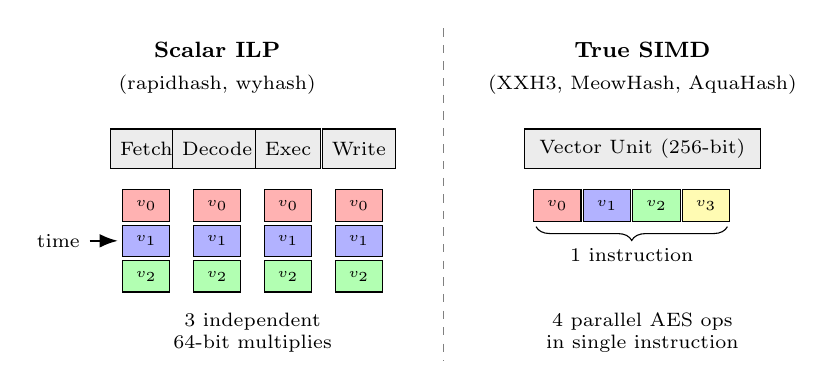
\begin{tikzpicture}[
    >=Latex,
    scale=0.9,
    inst/.style={rectangle, draw, minimum width=0.6cm, minimum height=0.4cm, font=\tiny},
    unit/.style={rectangle, draw, minimum width=0.7cm, minimum height=0.5cm, font=\scriptsize, fill=gray!15},
    label/.style={font=\scriptsize}
]
% === Scalar ILP (left side) ===
\node[label, font=\footnotesize\bfseries] at (0, 2.2) {Scalar ILP};
\node[label] at (0, 1.7) {(rapidhash, wyhash)};

% Pipeline stages
\node[unit] (f1) at (-1, 0.8) {Fetch};
\node[unit] (d1) at (0, 0.8) {Decode};
\node[unit] (e1) at (1, 0.8) {Exec};
\node[unit] (w1) at (2, 0.8) {Write};

% Instructions flowing through (3 independent chains)
\node[inst, fill=red!30] (i1a) at (-1, 0) {$v_0$};
\node[inst, fill=blue!30] (i2a) at (-1, -0.5) {$v_1$};
\node[inst, fill=green!30] (i3a) at (-1, -1) {$v_2$};

\node[inst, fill=red!30] (i1b) at (0, 0) {$v_0$};
\node[inst, fill=blue!30] (i2b) at (0, -0.5) {$v_1$};
\node[inst, fill=green!30] (i3b) at (0, -1) {$v_2$};

\node[inst, fill=red!30] (i1c) at (1, 0) {$v_0$};
\node[inst, fill=blue!30] (i2c) at (1, -0.5) {$v_1$};
\node[inst, fill=green!30] (i3c) at (1, -1) {$v_2$};

\node[inst, fill=red!30] (i1d) at (2, 0) {$v_0$};
\node[inst, fill=blue!30] (i2d) at (2, -0.5) {$v_1$};
\node[inst, fill=green!30] (i3d) at (2, -1) {$v_2$};

\draw[->, thick] (-1.8, -0.5) -- (-1.4, -0.5);
\node[label, anchor=east] at (-1.8, -0.5) {time};

\node[label, align=center] at (0.5, -1.8) {3 independent\\64-bit multiplies};

% === True SIMD (right side) ===
\node[label, font=\footnotesize\bfseries] at (6, 2.2) {True SIMD};
\node[label] at (6, 1.7) {(XXH3, MeowHash, AquaHash)};

% Vector unit
\node[unit, minimum width=3cm] (vu) at (6, 0.8) {Vector Unit (256-bit)};

% Single wide instruction
\node[inst, fill=red!30, minimum width=0.6cm] (s1) at (4.8, 0) {$v_0$};
\node[inst, fill=blue!30, minimum width=0.6cm] (s2) at (5.5, 0) {$v_1$};
\node[inst, fill=green!30, minimum width=0.6cm] (s3) at (6.2, 0) {$v_2$};
\node[inst, fill=yellow!30, minimum width=0.6cm] (s4) at (6.9, 0) {$v_3$};

\draw[decorate, decoration={brace, amplitude=5pt, mirror}] (4.5, -0.3) -- (7.2, -0.3);
\node[label] at (5.85, -0.7) {1 instruction};

\node[label, align=center] at (6, -1.8) {4 parallel AES ops\\in single instruction};

% Dividing line
\draw[dashed, gray] (3.2, 2.5) -- (3.2, -2.2);
\end{tikzpicture}
\end{center}

%=============================================================================
\section{Round Functions and Combiners}
%=============================================================================

This section details specific mixing functions used by hash families.
For the core primitives (MUM, ARX, etc.), see Section~\ref{sec:primitives}.

\subsection{The MUM Primitive}
\label{sec:mum}

\begin{center}
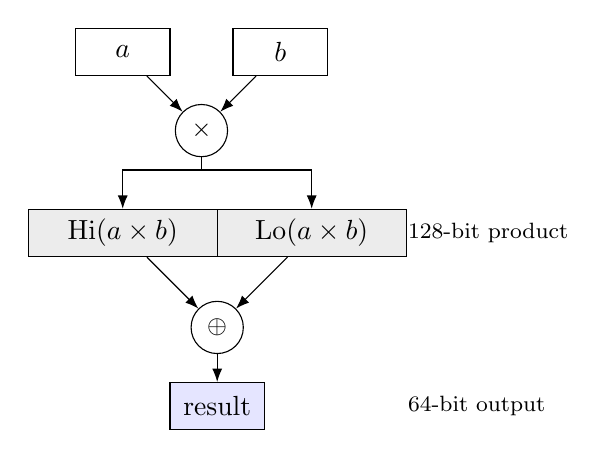
\begin{tikzpicture}[
    >=Latex,
    input/.style={rectangle, draw, minimum width=1.2cm, minimum height=0.6cm},
    output/.style={rectangle, draw, minimum width=2.4cm, minimum height=0.6cm, fill=gray!15},
    op/.style={circle, draw, minimum size=0.6cm, font=\small}
]
% Inputs
\node[input] (a) at (0,0) {$a$};
\node[input] (b) at (2,0) {$b$};

% Multiply
\node[op] (mul) at (1,-1) {$\times$};
\draw[->] (a) -- (mul);
\draw[->] (b) -- (mul);

% 128-bit result
\node[output] (hi) at (0,-2.3) {Hi$(a \times b)$};
\node[output] (lo) at (2.4,-2.3) {Lo$(a \times b)$};
\draw[->] (mul) -- ++(0,-0.5) -| (hi);
\draw[->] (mul) -- ++(0,-0.5) -| (lo);

% XOR fold
\node[op] (xor) at (1.2,-3.5) {$\oplus$};
\draw[->] (hi) -- (xor);
\draw[->] (lo) -- (xor);

% Output
\node[input, fill=blue!10] (out) at (1.2,-4.5) {result};
\draw[->] (xor) -- (out);

\node[anchor=west, font=\footnotesize] at (3.5,-2.3) {128-bit product};
\node[anchor=west, font=\footnotesize] at (3.5,-4.5) {64-bit output};
\end{tikzpicture}
\end{center}

We define three variants used throughout this survey:

\begin{description}
\item[$\Mum(a,\,b)$] \textbf{Standard (folded):} Returns $\textsc{Lo}(a \times b) \oplus \textsc{Hi}(a \times b)$.
Used by wyhash (\texttt{\_wymix}), rapidhash (\texttt{rapid\_mix}), XXH3.

\item[$\Mum^*(a,b)$] \textbf{Protected (folded):} XORs the original inputs back into the product
before folding, preventing degenerate cases (e.g.\ $a{=}0$) from collapsing state:
\begin{equation}
\Mum^*(a, b) = a \oplus b \oplus \textsc{Lo}(a \times b) \oplus \textsc{Hi}(a \times b)
\end{equation}
Used by wyhash-strict, rapidhash-protected, MuseAir.

\item[$\Mum_{128}(a,b)$] \textbf{Full product:} Returns the pair $(\textsc{Lo}(a \times b),\, \textsc{Hi}(a \times b))$
without folding. Used in finalizations where both halves update separate state variables.
\item[$\Mum_{128}^*(a,b)$] \textbf{Protected full product:} Returns the pair
$(a \oplus \textsc{Lo}(a \times b),\, b \oplus \textsc{Hi}(a \times b))$.
Folding this pair with XOR gives $\Mum^*(a,b)$.
\end{description}

\subsection{Round Functions}
\label{sec:round}

Many hashes use a \emph{round function} that mixes input into an accumulator.
The xxHash round functions are defined in Section~\ref{sec:xxhash-round}.

\subsection{Xorshift}
\label{sec:xorshift}

The xorshift primitive XORs a value with a shifted copy of itself:
\begin{equation}
\textsc{Xorshift}_r(v) = v \oplus (v \gg r)
\end{equation}

\paragraph{Permutation proof.}
$\textsc{Xorshift}_r$ is a bijection (permutation) for any $0 < r < w$ where $w$ is the word size.
To see this, note that the top $r$ bits of $v$ are unchanged, and each subsequent bit can be
recovered by XORing with the already-recovered bit $r$ positions above it. Equivalently,
applying $\textsc{Xorshift}_r$ a total of $\lceil w/r \rceil$ times yields the identity.

\subsection{ShiftMix}
\label{sec:shiftmix}

A specific xorshift used by CityHash and FarmHash:
\begin{equation}
\textsc{ShiftMix}(v) = \Xorshift{47}(v) = v \oplus (v \gg 47)
\end{equation}
This diffuses high bits into the low 17 bits of a 64-bit value.

\subsection{HashLen16 (CityHash)}
\label{sec:hashlen16}

CityHash's core 128-to-64 bit reducer, inspired by MurmurHash:

\begin{align}
a &\gets (u \oplus v) \cdot \mathit{mul} \\
a &\gets \ShiftMix(a) \\
b &\gets (v \oplus a) \cdot \mathit{mul} \\
b &\gets \ShiftMix(b) \\
\textsc{HashLen16}(u, v, \mathit{mul}) &\gets b \cdot \mathit{mul}
\end{align}
where $\mathit{mul}$ is an odd 64-bit multiplier (often a fixed constant, or $k_2 + 2n$ for length-dependent mixing).
When the multiplier is the fixed default, we may omit it and write $\textsc{HashLen16}(u, v)$.
This resembles \Mum{} but applies the shifts between multiplications rather than using 128-bit product folding.

\subsection{Finalization Mixers}
\label{sec:fmix}

All finalization mixers follow a common pattern: alternating xorshift and multiply operations.
The general form is:
\begin{align}
h &\gets \Xorshift{r_1}(h) \\
h &\gets h \cdot c_1 \\
h &\gets \Xorshift{r_2}(h) \\
h &\gets h \cdot c_2 \\
\textsc{fmix}(h) &\gets \Xorshift{r_3}(h)
\end{align}

Different hashes choose different shift amounts $(r_1, r_2, r_3)$ and multiplier constants $(c_1, c_2)$
based on avalanche analysis. Typical 32-bit shifts: $(16, 13, 16)$. Typical 64-bit shifts: $(33, 33, 33)$ or $(33, 29, 32)$.

This is a bijection: each $\Xorshift{r}$ is a permutation (see Section~\ref{sec:xorshift}),
and multiplication by an odd constant is a permutation mod $2^w$.

%=============================================================================
\section{The wyhash/rapidhash Family}
%=============================================================================

This family uses the MUM primitive as its core operation:
\begin{equation}
\Mum(a,\, b) = \textsc{Lo}(a \times b) \oplus \textsc{Hi}(a \times b)
\end{equation}

\subsection{Secrets}
\label{sec:wyconst}

Both families use 64-bit ``secret'' constants $s_0, s_1, \ldots$ for mixing.
wyhash uses 4 secrets; rapidhash uses 8 (the first 4 shared with wyhash).

\subsection{wyhash (64-bit)}
\label{sec:wyhash}

Source: \href{https://gitlab.com/fwojcik/smhasher3/-/blob/main/hashes/wyhash.cpp}{\texttt{hashes/wyhash.cpp}}~\cite{wyhash}.

\paragraph{SMHasher3 test results.}
wyhash fails 15 of 250 tests: Permutation tests with single-bit keys at all block sizes
(4--16 bytes, both LE and BE), and SeedZeroes at 1280 and 8448 bytes.
The Permutation failures reflect insufficient diffusion when only one bit of each input
word is set.

The main loop uses 3 scalar lanes (not 4 or 8) because \Mum{} relies on 64$\times$64$\to$128-bit
scalar multiplication, which doesn't vectorize in SSE/AVX. The 3 independent dependency chains
exploit ILP while keeping register pressure manageable.

\begin{algorithmic}[1]
\State $v_0 \gets \mathit{seed} \oplus \Mum(\mathit{seed} \oplus s_0,\, s_1)$
\For{$i \in \{1,2\}$}
    \State $v_i \gets v_0$
\EndFor
\For{each block $(x_0, \ldots, x_5)\in \ut{64}^6$} \Comment{Main loop: 3 parallel lanes}
    \For{$i \in \{0,1,2\}$}
        \State $v_i \gets \Mum(x_{2i} \oplus s_{i+1},\, x_{2i+1} \oplus v_i)$
    \EndFor
\EndFor
\State $v_0 \gets v_0 \oplus v_1 \oplus v_2$ \Comment{Collapse lanes}
\State Process remaining bytes; read last 16 bytes as $t_0, t_1$
\State $t_0 \gets t_0 \oplus s_1$, \quad $t_1 \gets t_1 \oplus v_0$
\State $(t_0, t_1) \gets (\textsc{Lo}(t_0 \times t_1), \textsc{Hi}(t_0 \times t_1))$
\State \Return $\Mum(t_0 \oplus s_0 \oplus n,\, t_1 \oplus s_1)$
\end{algorithmic}

\subsection{rapidhash}
\label{sec:rapidhash}

Source: \href{https://gitlab.com/fwojcik/smhasher3/-/blob/main/hashes/rapidhash.cpp}{\texttt{hashes/rapidhash.cpp}}, version 3~\cite{rapidhash}.

By Nicolas De Carli, based on wyhash. Uses 7 scalar ILP lanes (112-byte blocks), trading higher
register pressure for more parallelism on wide superscalar CPUs. Uses $s_2$ for seed initialization
and 8 secrets ($s_0$--$s_7$).

The ``protected'' variant XORs the original inputs back into the MUM result:
\begin{equation}
\Mum_{128}^*(a, b) = (a \oplus \textsc{Lo}(a \times b), \; b \oplus \textsc{Hi}(a \times b))
\end{equation}
This prevents zero-multiplication weaknesses at a small performance cost.

\begin{algorithmic}[1]
\State $v_0 \gets \mathit{seed} \oplus \Mum(\mathit{seed} \oplus s_2,\, s_1)$ \Comment{Note: $s_2$ not $s_0$}
\For{$i \in \{1,\ldots,6\}$}
    \State $v_i \gets v_0$
\EndFor
\For{each block $(x_0, \ldots, x_{13})\in \ut{64}^{14}$} \Comment{Main loop: 7 parallel lanes}
    \For{$i \in \{0,\ldots,6\}$}
        \State $v_i \gets \Mum(x_{2i} \oplus s_i,\, x_{2i+1} \oplus v_i)$
    \EndFor
\EndFor
\State $v_0 \gets v_0 \oplus v_1$; $v_2 \gets v_2 \oplus v_3$; $v_4 \gets v_4 \oplus v_5$ \Comment{Collapse lanes}
\State $v_0 \gets v_0 \oplus v_6$; $v_2 \gets v_2 \oplus v_4$; $v_0 \gets v_0 \oplus v_2$
\State Process remaining bytes; read last 16 bytes as $t_0, t_1$ with $t_0 \gets t_0 \oplus n$
\State $t_0 \gets t_0 \oplus s_1$, \quad $t_1 \gets t_1 \oplus v_0$
\State $(t_0, t_1) \gets (\textsc{Lo}(t_0 \times t_1), \textsc{Hi}(t_0 \times t_1))$
\State \Return $\Mum(t_0 \oplus s_7,\, t_1 \oplus s_1 \oplus n)$ \Comment{Note: $s_7$ and extra $n$}
\end{algorithmic}

\paragraph{XOR-tree lane combination:}

\begin{center}
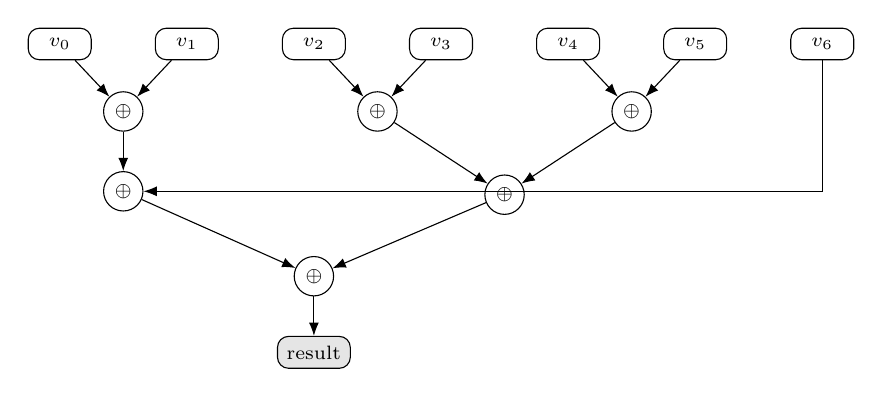
\begin{tikzpicture}[
    node distance=0.6cm and 0.8cm,
    xornode/.style={circle, draw, minimum size=0.5cm, inner sep=0pt, font=\scriptsize},
    lanenode/.style={rectangle, draw, rounded corners, minimum width=0.8cm, minimum height=0.4cm, font=\scriptsize}
]
% Initial lanes
\node[lanenode] (s0) {$v_0$};
\node[lanenode, right=of s0] (s1) {$v_1$};
\node[lanenode, right=of s1] (s2) {$v_2$};
\node[lanenode, right=of s2] (s3) {$v_3$};
\node[lanenode, right=of s3] (s4) {$v_4$};
\node[lanenode, right=of s4] (s5) {$v_5$};
\node[lanenode, right=of s5] (s6) {$v_6$};

% Level 1 XORs
\node[xornode, below=of $(s0)!0.5!(s1)$] (x1) {$\oplus$};
\node[xornode, below=of $(s2)!0.5!(s3)$] (x2) {$\oplus$};
\node[xornode, below=of $(s4)!0.5!(s5)$] (x3) {$\oplus$};

\draw[-Latex] (s0) -- (x1);
\draw[-Latex] (s1) -- (x1);
\draw[-Latex] (s2) -- (x2);
\draw[-Latex] (s3) -- (x2);
\draw[-Latex] (s4) -- (x3);
\draw[-Latex] (s5) -- (x3);

% Level 1.5 - v6 joins v0
\node[xornode, below=0.5cm of x1] (x1b) {$\oplus$};
\draw[-Latex] (x1) -- (x1b);
\draw[-Latex] (s6) |- (x1b);

% Level 2 XOR
\node[xornode, below=0.8cm of $(x2)!0.5!(x3)$] (x4) {$\oplus$};
\draw[-Latex] (x2) -- (x4);
\draw[-Latex] (x3) -- (x4);

% Final XOR
\node[xornode, below=0.8cm of $(x1b)!0.5!(x4)$] (xf) {$\oplus$};
\draw[-Latex] (x1b) -- (xf);
\draw[-Latex] (x4) -- (xf);

% Output
\node[lanenode, below=0.5cm of xf, fill=gray!20] (out) {result};
\draw[-Latex] (xf) -- (out);
\end{tikzpicture}
\end{center}

\paragraph{Tail (17--112 bytes).}
Nested conditionals process 16 bytes at a time with alternating secrets:
\begin{center}
\begin{tabular}{ccc}
\toprule
Bytes remaining & Offset & Secret \\
\midrule
$> 16$ & 0, 8 & $s_2$ \\
$> 32$ & 16, 24 & $s_2$ \\
$> 48$ & 32, 40 & $s_1$ \\
$> 64$ & 48, 56 & $s_1$ \\
$> 80$ & 64, 72 & $s_2$ \\
$> 96$ & 80, 88 & $s_1$ \\
\bottomrule
\end{tabular}
\end{center}

\paragraph{Finalization.}
Read last 16 bytes as $(t_0, t_1)$ with $t_0 \gets t_0 \oplus n$, then apply
$t_0 \gets t_0 \oplus s_1$, $t_1 \gets t_1 \oplus v_0$, and
$(t_0, t_1) \gets (\textsc{Lo}(t_0 \times t_1), \textsc{Hi}(t_0 \times t_1))$.
Return $\Mum(t_0 \oplus s_7,\, t_1 \oplus s_1 \oplus n)$.
Differs from wyhash: length is XORed into $a$ before MUM (not the final result),
uses $s_7$ instead of $s_0$, and includes length twice in finalization.

\subsection{rapidhash Variants}

\begin{center}
\begin{tabular}{lccc}
\toprule
Variant & Chunk size & Lanes & Secrets used \\
\midrule
rapidhash & 112 bytes & 7 & $s_0$--$s_7$ \\
rapidhashMicro & 80 bytes & 5 & $s_0$--$s_4$, $s_7$ \\
rapidhashNano & 48 bytes & 3 & $s_0$--$s_2$, $s_7$ \\
\bottomrule
\end{tabular}
\end{center}

\paragraph{Rust port.} The \texttt{rust-rapidhash} implementation uses a different
seed initialization: secrets are regenerated from the user seed using the protected
MUM variant, ensuring non-zero quality in specific bit ranges. This makes hashes
incompatible between the C and Rust versions for the same seed.

%=============================================================================
\section{The a5hash/MuseAir Family}
%=============================================================================

These hashes also use the MUM primitive but with different architectural choices
than wyhash/rapidhash.

\subsection{a5hash}
\label{sec:a5hash}

Source: \href{https://gitlab.com/fwojcik/smhasher3/-/blob/main/hashes/a5hash.cpp}{\texttt{hashes/a5hash.cpp}}, version 5.21~\cite{a5hash}.

A MUM-based hash by Aleksey Vaneev with a single MUM lane in the main loop (simpler than
wyhash's 3 lanes). Uses mantissa bits of $\pi$ for initial state and checkerboard masks
$c_0 = \texttt{0x5555...}$, $c_1 = \texttt{0xAAAA...}$ that ensure different bit positions
are treated differently. Addition of masks after each round prevents zero-multiplication
weaknesses. Available in 32-bit, 64-bit, and 128-bit variants.

\begin{algorithmic}[1]
\State $v_0 \gets \texttt{0x243F6A8885A308D3} \oplus n$, $v_1 \gets \texttt{0x452821E638D01377} \oplus n$ \Comment{From $\pi$}
\State $(v_0, v_1) \gets \Mum_{128}(v_1 \oplus (\mathit{seed} \land c_1), v_0 \oplus (\mathit{seed} \land c_0))$
\If{$n > 16$}
    \State $c_0 \gets c_0 \oplus v_0$; $c_1 \gets c_1 \oplus v_1$
    \For{each block $(x_0, x_1)\in \ut{64}^2$ excluding final 16 bytes} \Comment{Main loop}
        \State $(v_0, v_1) \gets \Mum_{128}(x_0 \oplus v_0, x_1 \oplus v_1)$
        \State $v_0 \gets v_0 + c_0$; $v_1 \gets v_1 + c_1$
    \EndFor
\EndIf
\State Handle tail (0--16 bytes) with overlapping reads
\State $(v_0, v_1) \gets \Mum_{128}(v_0, v_1)$
\State $(v_0, v_1) \gets \Mum_{128}(v_0 \oplus c_0, v_1)$
\State \Return $v_0 \oplus v_1$
\end{algorithmic}

Here $\Mum_{128}(a, b)$ returns both halves of the 128-bit product: $(\textsc{Lo}(a \times b), \textsc{Hi}(a \times b))$.

\subsection{MuseAir}
\label{sec:museair}

Source: \href{https://gitlab.com/fwojcik/smhasher3/-/blob/main/hashes/museair.cpp}{\texttt{hashes/museair.cpp}}, version 0.3~\cite{museair}.

A MUM-based hash by K--Aethiax with 6-lane parallelism and chained dependencies between lanes.
Uses 7 constants from $\mathrm{Ai}(0)$ mantissa ($s_0 = \texttt{0x5ae31e589c56e17a}$, ...).
The \hyperref[fn:museair-mumix]{\textsc{mumix}} primitive either XORs MUM output into state (standard) or replaces it (bfast).
Cross-lane MUM pattern in the epilogue ensures full mixing. Available in standard, bfast
(faster, slightly weaker), and 128-bit variants.

\paragraph{\hyperref[fn:museair-mumix]{\textsc{mumix}}.}\phantomsection\label{fn:museair-mumix}

\begin{algorithmic}[1]
\Function{mumix}{$v_p, v_q, x_p, x_q$} \Comment{State words $(v_p, v_q)$, input words $(x_p, x_q)$}
    \State $a \gets v_p \oplus x_p$; \quad $b \gets v_q \oplus x_q$
    \State $(\ell, h) \gets \Mum_{128}(a, b)$
    \State $(v_p, v_q) \gets (a \oplus \ell,\, b \oplus h)$ \Comment{Standard variant}
    \State \Comment{bfast variant: $(v_p, v_q) \gets (\ell,\, h)$}
\EndFunction
\end{algorithmic}

\paragraph{Long Keys.}

	\begin{algorithmic}[1]
	\State Initialize 6 state variables from seed:
	\State \quad $v_0 \gets s_0 + \mathit{seed}$, $v_1 \gets s_1 - \mathit{seed}$, $v_2 \gets s_2 \oplus \mathit{seed}$
	\State \quad $v_3 \gets s_3 + \mathit{seed}$, $v_4 \gets s_4 - \mathit{seed}$, $v_5 \gets s_5 \oplus \mathit{seed}$
	\State $t \gets s_6$ \Comment{Initial chain value}
	\For{each block $(x_0, \ldots, x_{11})\in \ut{64}^{12}$} \Comment{Main loop: 6 parallel lanes}
	    \For{$i \in \{0, \ldots, 5\}$}
	        \State $v_i \gets v_i \oplus x_{2i}$
	        \State $v_{(i+1) \bmod 6} \gets v_{(i+1) \bmod 6} \oplus x_{2i+1}$
	        \State $(\mathit{lo}, \mathit{hi}) \gets \Mum_{128}(v_i, v_{(i+1) \bmod 6})$
	        \State $v_i \gets v_i + (t \oplus \mathit{hi})$ \Comment{Chain: previous lo XOR current hi}
	        \State $t \gets \mathit{lo}$
	    \EndFor
	\EndFor
	\State $v_0 \gets v_0 + t$ \Comment{Fold in last chain value}
	\State Process remaining 48, 32, 16 bytes with \hyperref[fn:museair-mumix]{\textsc{mumix}}
	\State Apply \hyperref[fn:museair-mumix]{\textsc{mumix}} to the last 16 bytes (tail summarized)
	\State $t_0 \gets v_0 - v_1$, $t_1 \gets v_2 - v_3$, $t_2 \gets v_4 - v_5$ \Comment{Finalization: collapse lanes}
	\State $t_0 \gets \Rot{n \bmod 64}{t_0}$, $t_1 \gets \Rot{64-(n \bmod 64)}{t_1}$, $t_2 \gets t_2 \oplus n$ \Comment{$\Rot{64-r}{}$ is right-rotate by $r$}
	\State $(t'_0, t'_1) \gets \Mum_{128}(t_0, t_1)$, $(t'_2, t'_3) \gets \Mum_{128}(t_1, t_2)$, $(t'_4, t'_5) \gets \Mum_{128}(t_2, t_0)$
	\State $t_0 \gets t'_0 \oplus t'_5$, $t_1 \gets t'_2 \oplus t'_1$, $t_2 \gets t'_4 \oplus t'_3$ \Comment{Cross lo/hi}
	\State $(u_0, u_1) \gets \Mum_{128}(t_0, t_1)$, $(u_2, u_3) \gets \Mum_{128}(t_1, t_2)$, $(u_4, u_5) \gets \Mum_{128}(t_2, t_0)$
	\State \Return $(u_0 \oplus u_5) + (u_2 \oplus u_1) + (u_4 \oplus u_3)$ \Comment{64-bit}
	\end{algorithmic}

\begin{figure}[ht]
\centering
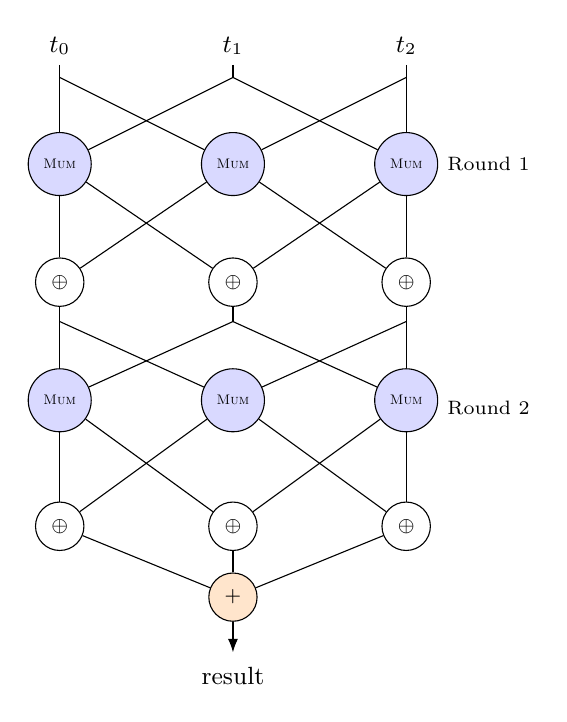
\begin{tikzpicture}[
    >=Latex,
    var/.style={font=\small},
    mum/.style={circle, draw, fill=blue!15, minimum size=0.8cm, font=\tiny, align=center},
    xornode/.style={circle, draw, minimum size=0.45cm, font=\scriptsize}
]
% Column positions (wider spacing)
\def\colA{0}
\def\colB{2.2}
\def\colC{4.4}

% === Row 0: Variables t_0, t_1, t_2 ===
\node[var] (i0) at (\colA, 0) {$t_0$};
\node[var] (j0) at (\colB, 0) {$t_1$};
\node[var] (k0) at (\colC, 0) {$t_2$};

% Vertical lines down from variables
\draw (i0) -- (\colA, -0.4);
\draw (j0) -- (\colB, -0.4);
\draw (k0) -- (\colC, -0.4);

% === Round 1: Mum nodes ===
\node[mum] (m1L) at (\colA, -1.5) {\textsc{Mum}};
\node[mum] (m1M) at (\colB, -1.5) {\textsc{Mum}};
\node[mum] (m1R) at (\colC, -1.5) {\textsc{Mum}};

% Lines to Mum nodes
\draw (\colA, -0.4) -- (m1L);
\draw (\colB, -0.4) -- (m1L);
\draw (\colB, -0.4) -- (m1R);
\draw (\colC, -0.4) -- (m1R);
\draw (\colA, -0.4) -- (m1M);
\draw (\colC, -0.4) -- (m1M);

% === XOR nodes (after Round 1) ===
\node[xornode] (xor1a) at (\colA, -3.0) {$\oplus$};
\node[xornode] (xor1b) at (\colB, -3.0) {$\oplus$};
\node[xornode] (xor1c) at (\colC, -3.0) {$\oplus$};

% Lines from Mum to XOR
\draw (m1L) -- (xor1a);
\draw (m1L) -- (xor1b);
\draw (m1M) -- (xor1a);
\draw (m1M) -- (xor1c);
\draw (m1R) -- (xor1b);
\draw (m1R) -- (xor1c);

% Vertical lines after XOR
\draw (xor1a) -- (\colA, -3.5);
\draw (xor1b) -- (\colB, -3.5);
\draw (xor1c) -- (\colC, -3.5);

% === Round 2: Mum nodes ===
\node[mum] (m2L) at (\colA, -4.5) {\textsc{Mum}};
\node[mum] (m2M) at (\colB, -4.5) {\textsc{Mum}};
\node[mum] (m2R) at (\colC, -4.5) {\textsc{Mum}};

% Lines to Mum nodes
\draw (\colA, -3.5) -- (m2L);
\draw (\colB, -3.5) -- (m2L);
\draw (\colB, -3.5) -- (m2R);
\draw (\colC, -3.5) -- (m2R);
\draw (\colA, -3.5) -- (m2M);
\draw (\colC, -3.5) -- (m2M);

% === XOR nodes (after Round 2) ===
\node[xornode] (xor2a) at (\colA, -6.1) {$\oplus$};
\node[xornode] (xor2b) at (\colB, -6.1) {$\oplus$};
\node[xornode] (xor2c) at (\colC, -6.1) {$\oplus$};

% Lines from Mum to XOR
\draw (m2L) -- (xor2a);
\draw (m2L) -- (xor2b);
\draw (m2M) -- (xor2a);
\draw (m2M) -- (xor2c);
\draw (m2R) -- (xor2b);
\draw (m2R) -- (xor2c);

% === Converge to sum ===
\node[xornode, fill=orange!20] (sum) at (\colB, -7.0) {$+$};
\draw (xor2a) -- (sum);
\draw (xor2b) -- (sum);
\draw (xor2c) -- (sum);

% === Result ===
\draw[->] (sum) -- (\colB, -7.7);
\node[var] at (\colB, -8.0) {result};

% Round labels
\node[font=\scriptsize, anchor=west] at (4.8, -1.5) {Round 1};
\node[font=\scriptsize, anchor=west] at (4.8, -4.6) {Round 2};

\end{tikzpicture}
\caption{MuseAir finalizer. Each round performs three $\Mum_{128}$ operations on all pairs of its three inputs, then cross-XORs the lo/hi halves. After two rounds the three values are summed for the 64-bit result.}
\label{fig:museair-finalizer}
\end{figure}

%=============================================================================
\section{xxHash Family}
%=============================================================================

Source: \href{https://gitlab.com/fwojcik/smhasher3/-/blob/main/hashes/xxhash.cpp}{\texttt{hashes/xxhash.cpp}}~\cite{xxhash}.

xxHash uses prime constants $s_1, \ldots, s_5$ selected by empirical testing for
avalanche properties. The primes have roughly half their bits set and avoid
degenerate bit patterns. For xxHash64:
\begin{align*}
s_1 &= \texttt{0x9E3779B185EBCA87} & s_2 &= \texttt{0xC2B2AE3D27D4EB4F} \\
s_3 &= \texttt{0x165667B19E3779F9} & s_4 &= \texttt{0x85EBCA77C2B2AE63} \\
s_5 &= \texttt{0x27D4EB2F165667C5}
\end{align*}
The 32-bit versions use corresponding 32-bit primes.

\subsection{Round Functions}

\subsubsection{Multiply-Rotate Round}
\label{sec:xxhash-round}

The xxHash round function mixes input into an accumulator:

\begin{equation}
\textsc{Round}(v, x) = \Rot{r}{v + x \cdot s_2} \cdot s_1
\end{equation}
where $r = 13$ for 32-bit, $r = 31$ for 64-bit. This is an ARX variant
using multiplication instead of XOR for the final mix.

\subsubsection{Merge Round (xxHash64)}
\label{sec:merge}

After the main loop, xxHash64 merges each accumulator into the hash:
\begin{equation}
\textsc{Merge}(h, v) = (h \oplus \textsc{Round}(0, v)) \cdot s_1 + s_4
\end{equation}
This ``rounds'' the accumulator value, XORs it into the hash, then applies
another multiply-add for diffusion.

\paragraph{SMHasher3 test results.}
None of the xxHash variants pass the full SMHasher3 test battery.
xxHash32 fails 83 of 250 tests, including numerous Sparse, Permutation, and
seed-sensitivity tests (SeedBlockLen, SeedBlockOffset, SeedBIC, SeedBitflip),
reflecting the limited mixing of its 32-bit multiply-rotate round.
xxHash64 fares much better, failing only 9 tests, all seed-related
(SeedBlockLen, SeedBlockOffset, SeedBIC).
XXH3 (64-bit) fails 27 of 250 tests: BIC, Sparse, PerlinNoise, and Bitflip tests
expose weaknesses in the non-seeded path, while SeedZeroes produces 571 full
64-bit collisions (expected 0) on keys up to 1280 bytes with low-weight seeds---a
consequence of XXH3's seeding mechanism, which adds $\pm\mathit{seed}$ to the
secret and thus maps $\mathit{seed}=0$ and any seed that leaves all
relevant secret words unchanged to identical output.

\subsection{xxHash32}

\begin{algorithmic}[1]
\State $v_0 \gets \mathit{seed} + s_1 + s_2$
\State $v_1 \gets \mathit{seed} + s_2$
\State $v_2 \gets \mathit{seed}$
\State $v_3 \gets \mathit{seed} - s_1$
\If{$n \geq 16$}
    \For{each block $(x_0, x_1, x_2, x_3)\in \ut{32}^4$} \Comment{Main loop: 4 parallel lanes}
        \For{$i \in \{0,\ldots,3\}$}
            \State $v_i \gets \Round(v_i, x_i)$
        \EndFor
    \EndFor
    \State $v_4 \gets \Rot{1}{v_0} + \Rot{7}{v_1} + \Rot{12}{v_2} + \Rot{18}{v_3}$
\Else
    \State $v_4 \gets \mathit{seed} + s_5$
\EndIf
\State $v_4 \gets v_4 + n$
\For{each remaining $x_i \in \ut{32}$}
    \State $v_4 \gets \Rot{17}{v_4 + x_i \cdot s_3} \cdot s_4$
\EndFor
\For{each remaining $x_i \in \ut{8}$}
    \State $v_4 \gets \Rot{11}{v_4 + x_i \cdot s_5} \cdot s_1$
\EndFor
\State \Return $\hyperref[fn:xxh32-avalanche]{\textsc{XXH32\_avalanche}}(v_4)$
\end{algorithmic}

\paragraph{XXH32\_avalanche:}\phantomsection\label{fn:xxh32-avalanche} xxHash32 finalizer (an \textsc{XMS} cascade):
\begin{equation}
\textsc{XXH32\_avalanche}(h) = \Xorshift{16}\!\left(\textsc{XMS}_{13,s_3^{32}}\!\left(\textsc{XMS}_{15,s_2^{32}}(h)\right)\right)
\end{equation}

\subsection{xxHash64}

Same structure as xxHash32 with 64-bit words, $r=31$, and 32-byte blocks.

\begin{algorithmic}[1]
\State $v_0 \gets \mathit{seed} + s_1 + s_2$
\State $v_1 \gets \mathit{seed} + s_2$
\State $v_2 \gets \mathit{seed}$
\State $v_3 \gets \mathit{seed} - s_1$
\If{$n \geq 32$}
    \For{each block $(x_0, x_1, x_2, x_3)\in \ut{64}^4$} \Comment{Main loop: 4 parallel lanes}
        \For{$i \in \{0,\ldots,3\}$}
            \State $v_i \gets \Round(v_i, x_i)$
        \EndFor
    \EndFor
    \State $v_4 \gets \Rot{1}{v_0} + \Rot{7}{v_1} + \Rot{12}{v_2} + \Rot{18}{v_3}$
    \For{$i \in \{0,\ldots,3\}$}
        \State $v_4 \gets \Merge(v_4, v_i)$
    \EndFor
\Else
    \State $v_4 \gets \mathit{seed} + s_5$
\EndIf
\State $v_4 \gets v_4 + n$
\For{each remaining $x_i \in \ut{64}$}
    \State $v_4 \gets \Rot{27}{v_4 \oplus \Round(0, x_i)} \cdot s_1 + s_4$
\EndFor
\For{each remaining $x_i \in \ut{32}$}
    \State $v_4 \gets \Rot{23}{v_4 \oplus (x_i \cdot s_1)} \cdot s_2 + s_3$
\EndFor
\For{each remaining $x_i \in \ut{8}$}
    \State $v_4 \gets \Rot{11}{v_4 \oplus (x_i \cdot s_5)} \cdot s_1$
\EndFor
\State \Return $\hyperref[fn:xxh64-avalanche]{\textsc{XXH64\_avalanche}}(v_4)$
\end{algorithmic}

\paragraph{XXH64\_avalanche:}\phantomsection\label{fn:xxh64-avalanche} xxHash64 finalizer:
\begin{equation}
\textsc{XXH64\_avalanche}(h) = \Xorshift{32}\!\left(\textsc{XMS}_{29,s_3}\!\left(\textsc{XMS}_{33,s_2}(h)\right)\right)
\end{equation}

\subsection{XXH3}
\label{sec:xxh3}

Source: \href{https://gitlab.com/fwojcik/smhasher3/-/blob/main/hashes/xxhash.cpp}{\texttt{hashes/xxhash.cpp}}.

XXH3 (2019) uses a 192-byte secret $S$ (pseudorandom bytes from FARSH; seeded variant adds
$\pm\mathit{seed}$ to alternating 8-byte blocks). The 32$\times$32 multiply has native SIMD
support (unlike 64$\times$64). Original input is added to accumulators to prevent multiply-by-zero
weakness. Six distinct code paths optimize for different input sizes; short keys ($n \leq 240$)
use specialized scalar paths with 64$\times$64 MUM. We summarize those special cases and focus on the long-key path.

\paragraph{Long Keys ($n > 240$).}
\label{sec:xxh3-long}
Uses 8 parallel 64-bit accumulators with UMAC-inspired structure.

\paragraph{Accumulate (per 64-byte stripe).}

One stripe feeds 8 input words into 4 lane pairs.
Within each pair, the two lanes cross-pollinate: the raw input of each lane
is added to the \emph{other} lane's accumulator, hardening against multiply-by-zero.

\begin{center}
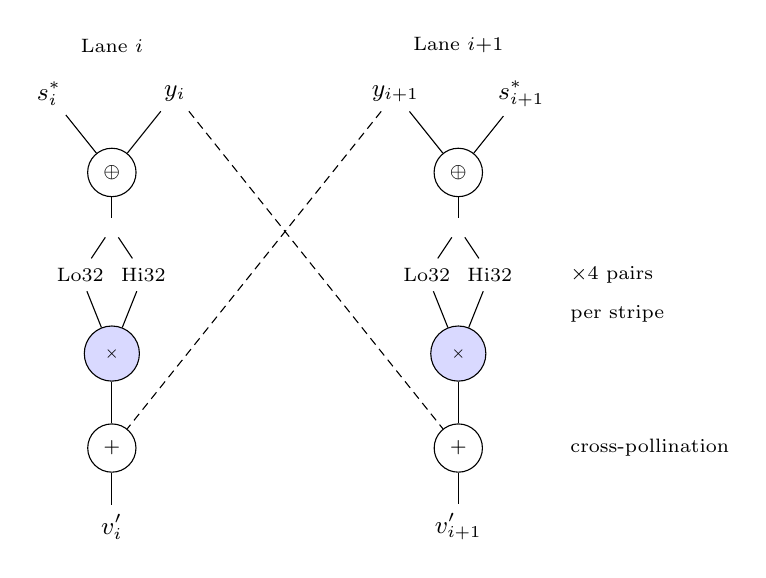
\begin{tikzpicture}[
    >=Latex,
    var/.style={font=\small},
    mul/.style={circle, draw, fill=blue!15, minimum size=0.7cm, font=\tiny, align=center},
    xornode/.style={circle, draw, minimum size=0.45cm, font=\scriptsize}
]
% Column positions
\def\colL{0}
\def\colR{4.4}

% === Row 0: Inputs ===
\node[var] (sL) at (\colL, 0) {$s^*_i$};
\node[var] (yL) at (\colL+1.6, 0) {$y_i$};
\node[var] (yR) at (\colR, 0) {$y_{i+1}$};
\node[var] (sR) at (\colR+1.6, 0) {$s^*_{i+1}$};

% === Row 1: XOR with secret ===
\node[xornode] (xorL) at (\colL+0.8, -1.0) {$\oplus$};
\node[xornode] (xorR) at (\colR+0.8, -1.0) {$\oplus$};
\draw (yL) -- (xorL);
\draw (sL) -- (xorL);
\draw (yR) -- (xorR);
\draw (sR) -- (xorR);

\node (xorLsouth) at (\colL+0.8, -1.7) {};
\node (xorRsouth) at (\colR+0.8, -1.7) {};
\draw (xorL) -- (xorLsouth);
\draw (xorR) -- (xorRsouth);

% === Row 2: Split in Lo/Hi 32 ===
\node[font=\scriptsize] (loL) at (\colL+0.4, -2.3) {Lo32};
\node[font=\scriptsize] (hiL) at (\colL+1.2, -2.3) {Hi32};
\node[font=\scriptsize] (loR) at (\colR+0.4, -2.3) {Lo32};
\node[font=\scriptsize] (hiR) at (\colR+1.2, -2.3) {Hi32};
\draw (xorLsouth) -- (loL);
\draw (xorLsouth) -- (hiL);
\draw (xorRsouth) -- (loR);
\draw (xorRsouth) -- (hiR);

% === Row 3: 32x32 multiply ===
\node[mul] (mulL) at (\colL+0.8, -3.3) {$\times$};
\node[mul] (mulR) at (\colR+0.8, -3.3) {$\times$};
\draw (loL) -- (mulL);
\draw (hiL) -- (mulL);
\draw (loR) -- (mulR);
\draw (hiR) -- (mulR);

% === Row 4: Add multiply result ===
\node[xornode] (addL) at (\colL+0.8, -4.5) {$+$};
\node[xornode] (addR) at (\colR+0.8, -4.5) {$+$};
\draw (mulL) -- (addL);
\draw (mulR) -- (addR);

% === Cross-pollination: raw input to other lane ===
\draw[densely dashed] (yL) -- (addR);
\draw[densely dashed] (yR) -- (addL);

% === Row 5: Outputs ===
\node[var] (vL2) at (\colL+0.8, -5.5) {$v'_i$};
\node[var] (vR2) at (\colR+0.8, -5.5) {$v'_{i+1}$};
\draw (addL) -- (vL2);
\draw (addR) -- (vR2);

% Lane labels
\node[font=\scriptsize, anchor=south] at (\colL+0.8, 0.4) {Lane $i$};
\node[font=\scriptsize, anchor=south] at (\colR+0.8, 0.4) {Lane $i{+}1$};

% Side label
\node[font=\scriptsize, anchor=west] at (6.5, -2.3) {$\times 4$ pairs};
\node[font=\scriptsize, anchor=west] at (6.5, -2.8) {per stripe};
\node[font=\scriptsize, anchor=west] at (6.5, -4.5) {cross-pollination};
\end{tikzpicture}
\end{center}

\noindent\textbf{Key insight}: The 32$\times$32$\to$64 multiply (not 64$\times$64!) enables efficient SIMD:
SSE2/AVX2 have \texttt{\_mm\_mul\_epu32} for this operation. The cross-lane addition
of original input (dashed lines) hardens against multiply-by-zero.

\begin{algorithmic}[1]
\State Initialize $(v_0, \ldots, v_7) \gets (s_3^{32}, s_1^{64}, s_2^{64}, s_3^{64}, s_4^{64}, s_2^{32}, s_5^{64}, s_1^{32})$
\State Let $s^{\mathrm{end}}_0, \ldots, s^{\mathrm{end}}_7$ be eight 64-bit secret words from the end of $S^\star$
\State Let $s^{\mathrm{m}}_0, \ldots, s^{\mathrm{m}}_7$ be eight 64-bit secret words from $S^\star$ at byte offset 11
\For{each block $(x_i)_{i=0}^{127} \in \ut{64}^{128}$} \Comment{1024 bytes = 16 stripes}
    \For{$j \in \{0, \ldots, 15\}$} \Comment{Stripe $j$ (64 bytes)}
        \State $(y_0,\ldots,y_7) \gets (x_{8j},\ldots,x_{8j+7})$
        \State Let $(s^*_0,\ldots,s^*_7)\in \ut{64}^8$ be the secret words for stripe $j$
        \For{$i \in \{0,\ldots,7\}$}
            \State $t \gets y_i \oplus s^*_i$ \Comment{32$\times$32 multiply of two halves (not MUM)}
            \State $v_i \gets v_i + (\textsc{Lo32}(t)\cdot \textsc{Hi32}(t))$
            \State $v_{i \oplus 1} \gets v_{i \oplus 1} + y_i$ \Comment{Cross-pollination: raw input}
        \EndFor
    \EndFor
    \For{$i \in \{0, \ldots, 7\}$} \Comment{Scramble accumulators}
        \State $v_i \gets (v_i \oplus (v_i \gg 47) \oplus s^{\mathrm{end}}_i) \cdot s_1^{32}$
    \EndFor
\EndFor
\State Handle remaining bytes (short/medium paths summarized)
\State $v \gets n \cdot s_1^{64}$ \Comment{Merge accumulators}
\For{$i \in \{0,2,4,6\}$}
    \State $v \gets v + \Mum(v_{i} \oplus s^{\mathrm{m}}_{i},\, v_{i+1} \oplus s^{\mathrm{m}}_{i+1})$
\EndFor
\State $v \gets v \oplus (v \gg 37)$ \Comment{Finalization (xorshift/multiply avalanche)}
\State $v \gets v \cdot \texttt{0x165667919E3779F9}$
\State \Return $v \oplus (v \gg 32)$
\end{algorithmic}

%=============================================================================
\section{SipHash Family}
%=============================================================================

Source: \href{https://gitlab.com/fwojcik/smhasher3/-/blob/main/hashes/siphash.cpp}{\texttt{hashes/siphash.cpp}}~\cite{siphash}.

SipHash is a cryptographically-informed hash function designed to resist hash-flooding DoS attacks.
Requires a 128-bit secret key. Uses an ARX construction (no multiplications) with a keyed permutation
and Feistel-like cross-lane mixing. Sequential by design---cannot be parallelized across blocks.

\subsection{Constants}

Initialization vectors $s_0, s_1, s_2, s_3$ are fixed 64-bit constants
(they encode the ASCII string ``somepseudorandomlygeneratedbytes'').

\subsection{SipRound}
\label{sec:sipround}

The core permutation operates on four 64-bit state words $(v_0, v_1, v_2, v_3)$.
It consists of two half-rounds with a cross-over in between:

\begin{center}
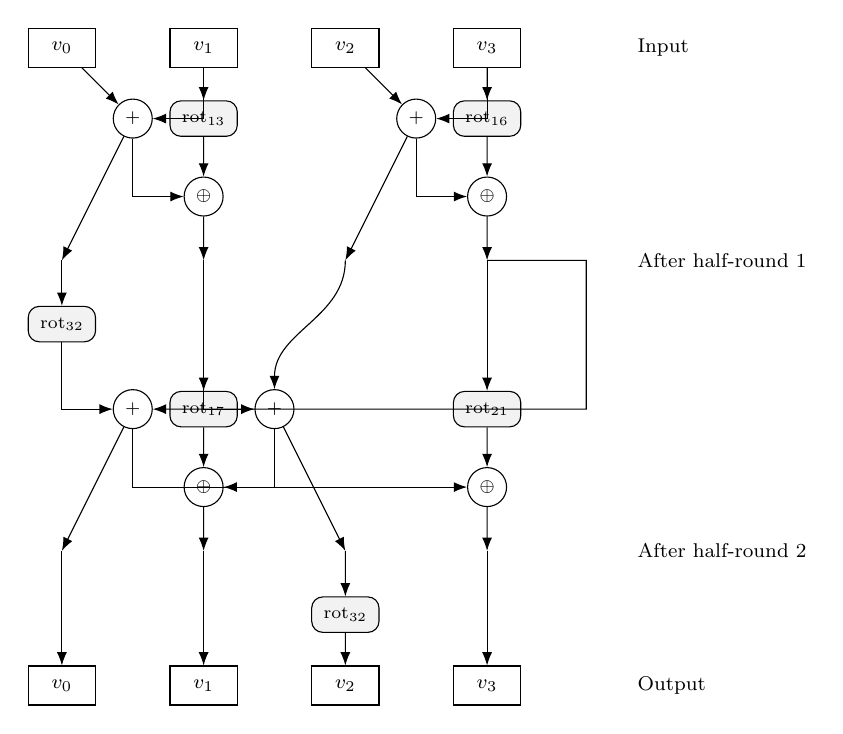
\begin{tikzpicture}[
    >=Latex,
    scale=0.9,
    transform shape,
    state/.style={rectangle, draw, minimum width=0.95cm, minimum height=0.55cm, font=\footnotesize},
    opnode/.style={circle, draw, minimum size=0.55cm, inner sep=0pt, font=\scriptsize},
    rotnode/.style={rectangle, draw, rounded corners, minimum width=0.95cm, minimum height=0.5cm, font=\scriptsize, fill=gray!10}
]
% Lanes
\def\xA{0}
\def\xB{2.0}
\def\xC{4.0}
\def\xD{6.0}
\def\xR{7.4}
\def\xL{-1.4}

% Rows
\def\yIn{0}
\def\yAddA{-1.0}
\def\yXorA{-2.1}
\def\yAfterA{-3.0}
\def\yRotA{-3.9}
\def\yAddB{-5.1}
\def\yXorB{-6.2}
\def\yAfterB{-7.1}
\def\yRotB{-8.0}
\def\yOut{-9.0}

% Input
\node[state] (in0) at (\xA,\yIn) {$v_0$};
\node[state] (in1) at (\xB,\yIn) {$v_1$};
\node[state] (in2) at (\xC,\yIn) {$v_2$};
\node[state] (in3) at (\xD,\yIn) {$v_3$};

% === Half-round 1 ===
% v0 += v1; v1 = rot13(v1) xor v0
\node[opnode]  (add01) at (1.0,\yAddA) {$+$};
\node[rotnode] (rot13) at (\xB,\yAddA) {rot$_{13}$};
\node[opnode]  (xor01) at (\xB,\yXorA) {$\oplus$};
\coordinate (v0a) at (\xA,\yAfterA);
\coordinate (v1a) at (\xB,\yAfterA);

\draw[->] (in0) -- (add01);
\draw[->] (in1) |- (add01);
\draw[->] (in1) -- (rot13);
\draw[->] (add01) -- (v0a);
\draw[->] (add01) |- (xor01);
\draw[->] (rot13) -- (xor01);
\draw[->] (xor01) -- (v1a);

% v2 += v3; v3 = rot16(v3) xor v2
\node[opnode]  (add23) at (5.0,\yAddA) {$+$};
\node[rotnode] (rot16) at (\xD,\yAddA) {rot$_{16}$};
\node[opnode]  (xor23) at (\xD,\yXorA) {$\oplus$};
\coordinate (v2a) at (\xC,\yAfterA);
\coordinate (v3a) at (\xD,\yAfterA);

\draw[->] (in2) -- (add23);
\draw[->] (in3) |- (add23);
\draw[->] (in3) -- (rot16);
\draw[->] (add23) -- (v2a);
\draw[->] (add23) |- (xor23);
\draw[->] (rot16) -- (xor23);
\draw[->] (xor23) -- (v3a);

% Cross-over: v0 = rot32(v0)
\node[rotnode] (rot32a) at (\xA,\yRotA) {rot$_{32}$};
\draw[->] (v0a) -- (rot32a);

% === Half-round 2 ===
% v2 += v1; v1 = rot17(v1) xor v2
\node[opnode]  (add21) at (3.0,\yAddB) {$+$};
\node[rotnode] (rot17) at (\xB,\yAddB) {rot$_{17}$};
\node[opnode]  (xor21) at (\xB,\yXorB) {$\oplus$};
\coordinate (v2b) at (\xC,\yAfterB);
\coordinate (v1b) at (\xB,\yAfterB);

\draw[->] (v2a) to[out=-90,in=90] (add21);
\draw[->] (v1a) |- (add21);
\draw[->] (v1a) -- (rot17);
\draw[->] (add21) -- (v2b);
\draw[->] (add21) |- (xor21);
\draw[->] (rot17) -- (xor21);
\draw[->] (xor21) -- (v1b);

% v0 += v3; v3 = rot21(v3) xor v0
\node[opnode]  (add03) at (1.0,\yAddB) {$+$};
\node[rotnode] (rot21) at (\xD,\yAddB) {rot$_{21}$};
\node[opnode]  (xor03) at (\xD,\yXorB) {$\oplus$};
\coordinate (v0b) at (\xA,\yAfterB);
\coordinate (v3b) at (\xD,\yAfterB);

\draw[->] (rot32a) |- (add03);
% Route v3 to add03 outside to avoid a central crossing.
\draw[->] (v3a) -- (\xR,\yAfterA) -- (\xR,\yAddB) -- (add03);
\draw[->] (v3a) -- (rot21);
\draw[->] (add03) -- (v0b);
\draw[->] (add03) |- (xor03);
\draw[->] (rot21) -- (xor03);
\draw[->] (xor03) -- (v3b);

% Final: v2 = rot32(v2)
\node[rotnode] (rot32b) at (\xC,\yRotB) {rot$_{32}$};
\draw[->] (v2b) -- (rot32b);

% Output
\node[state] (out0) at (\xA,\yOut) {$v_0$};
\node[state] (out1) at (\xB,\yOut) {$v_1$};
\node[state] (out2) at (\xC,\yOut) {$v_2$};
\node[state] (out3) at (\xD,\yOut) {$v_3$};

\draw[->] (v0b) -- (out0);
\draw[->] (v1b) -- (out1);
\draw[->] (rot32b) -- (out2);
\draw[->] (v3b) -- (out3);

% Stage labels
\node[font=\footnotesize,anchor=west] at (8.0,\yIn) {Input};
\node[font=\footnotesize,anchor=west] at (8.0,\yAfterA) {After half-round 1};
\node[font=\footnotesize,anchor=west] at (8.0,\yAfterB) {After half-round 2};
\node[font=\footnotesize,anchor=west] at (8.0,\yOut) {Output};
\end{tikzpicture}
\end{center}

\noindent Each half-round: $v_i \gets v_i + v_{i+1}$, then $v_{i+1} \gets \Rot{r}{v_{i+1}} \oplus v_i$.
After the first half-round, $v_0 \gets \Rot{32}{v_0}$ and the next half-round re-pairs the lanes to mix $(v_0, v_3)$ and $(v_2, v_1)$.
The second half-round uses rotations 17 and 21, followed by $v_2 \gets \Rot{32}{v_2}$.

\medskip
\noindent The complete algebraic form:
\begin{align}
v_0 &\gets v_0 + v_1 & v_2 &\gets v_2 + v_3 \\
v_1 &\gets \Rot{13}{v_1} & v_3 &\gets \Rot{16}{v_3} \\
v_1 &\gets v_1 \oplus v_0 & v_3 &\gets v_3 \oplus v_2 \\
v_0 &\gets \Rot{32}{v_0} \\
v_2 &\gets v_2 + v_1 & v_0 &\gets v_0 + v_3 \\
v_1 &\gets \Rot{17}{v_1} & v_3 &\gets \Rot{21}{v_3} \\
v_1 &\gets v_1 \oplus v_2 & v_3 &\gets v_3 \oplus v_0 \\
v_2 &\gets \Rot{32}{v_2}
\end{align}

\subsection{\texorpdfstring{SipHash-$c$-$d$}{SipHash-c-d}}
\label{sec:siphash}

Parameters $c$ and $d$ specify compression and finalization rounds.

\begin{algorithmic}[1]
\State $v_0 \gets k_0 \oplus s_0$
\State $v_1 \gets k_1 \oplus s_1$
\State $v_2 \gets k_0 \oplus s_2$
\State $v_3 \gets k_1 \oplus s_3$
\For{each block $x \in \ut{64}$}
    \State $v_3 \gets v_3 \oplus x$
    \For{$i \gets 1$ to $c$} \Comment{Compression rounds}
        \State \SipRound{}
    \EndFor
    \State $v_0 \gets v_0 \oplus x$
\EndFor
\State $x \gets$ padded final block with length byte
\State $v_3 \gets v_3 \oplus x$
\For{$i \gets 1$ to $c$} \Comment{Compression rounds}
    \State \SipRound{}
\EndFor
\State $v_0 \gets v_0 \oplus x$
\State $v_2 \gets v_2 \oplus \texttt{0xff}$
\For{$i \gets 1$ to $d$} \Comment{Finalization rounds}
    \State \SipRound{}
\EndFor
\State \Return $v_0 \oplus v_1 \oplus v_2 \oplus v_3$
\end{algorithmic}

\paragraph{Common variants:}
SipHash-2-4 ($c{=}2$, $d{=}4$): recommended.
SipHash-1-3 ($c{=}1$, $d{=}3$): faster, lower security margin.

\subsection{HalfSipHash}

32-bit variant for resource-constrained environments (used in Linux kernel).

\paragraph{SipRound (32-bit):}
Different rotation constants: $(5, 8, 7, 13, 16)$ instead of $(13, 16, 17, 21, 32)$.

%=============================================================================
\section{Other Notable Hashes}
%=============================================================================

%-----------------------------------------------------------------------------
\subsection{ARX-Based Hashes}
%-----------------------------------------------------------------------------

These hashes use Add-Rotate-XOR primitives without multiplication in their
main loops, relying on superscalar execution for parallelism.

\subsubsection{SpookyHash}
\label{sec:spookyhash}

Source: \href{https://gitlab.com/fwojcik/smhasher3/-/blob/main/hashes/spookyhash.cpp}{\texttt{hashes/spookyhash.cpp}}~\cite{spookyhash}.

By Bob Jenkins (creator of lookup3). A 128-bit ARX hash using 12 parallel
64-bit lanes with 96-byte blocks. Version 2 is most commonly used.

\paragraph{Mix Function.}\phantomsection\label{fn:spooky-mix}
The Mix function updates 12 state variables with 12 input words simultaneously.
Each line combines: word addition, cross-lane XOR, self-XOR, rotation, and
accumulation into adjacent lane. Rotations are: 11, 32, 43, 31, 17, 28, 39, 57, 55, 54, 22, 46.

\begin{center}
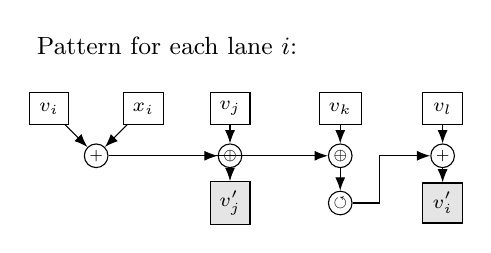
\begin{tikzpicture}[
    >=Latex,
    node distance=0.4cm,
    state/.style={rectangle, draw, minimum width=0.5cm, minimum height=0.4cm, font=\scriptsize},
    op/.style={circle, draw, minimum size=0.3cm, font=\tiny, inner sep=0pt}
]
% Show the pattern for one iteration
\node[font=\small] at (0, 1.2) {Pattern for each lane $i$:};
\node[state] (si) at (-1.5, 0.4) {$v_i$};
\node[state] (xi) at (-0.3, 0.4) {$x_i$};
\node[op] (add) at (-0.9, -0.2) {$+$};
\draw[->] (si) -- (add);
\draw[->] (xi) -- (add);

\node[state] (sj) at (0.8, 0.4) {$v_{j}$};
\node[op] (xor1) at (0.8, -0.2) {$\oplus$};
\draw[->] (add) -- (xor1);
\draw[->] (sj) -- (xor1);

\node[state, fill=gray!20] (sj2) at (0.8, -0.8) {$v'_{j}$};
\draw[->] (xor1) -- (sj2);

\node[state] (sk) at (2.2, 0.4) {$v_{k}$};
\node[op] (xor2) at (2.2, -0.2) {$\oplus$};
\draw[->] (add) -- ++(0.5,0) |- (xor2);
\draw[->] (sk) -- (xor2);

\node[op] (rot) at (2.2, -0.8) {$\circlearrowleft$};
\draw[->] (xor2) -- (rot);

\node[state] (sl) at (3.5, 0.4) {$v_{l}$};
\node[op] (add2) at (3.5, -0.2) {$+$};
\draw[->] (rot) -- ++(0.5,0) |- (add2);
\draw[->] (sl) -- (add2);

\node[state, fill=gray!20] (si2) at (3.5, -0.8) {$v'_{i}$};
\draw[->] (add2) -- (si2);
\end{tikzpicture}
\end{center}

Each of the 12 lanes follows this pattern with different rotation amounts and
cross-lane indices $j$, $k$, $l$.

\medskip
\noindent
Exact long-key round functions (SpookyHash v2):
\begin{algorithmic}[1]
\Function{Mix}{$x_0,\ldots,x_{11}, v_0,\ldots,v_{11}$} \Comment{96 bytes into 12 lanes}
    \State Let $(r_0,\ldots,r_{11}) \gets (11,32,43,31,17,28,39,57,55,54,22,46)$
    \For{$i \in \{0,\ldots,11\}$} \Comment{All indices mod 12}
        \State $v_i \gets v_i + x_i$
        \State $v_{(i+2)\bmod 12} \gets v_{(i+2)\bmod 12} \oplus v_{(i+10)\bmod 12}$
        \State $v_{(i+11)\bmod 12} \gets v_{(i+11)\bmod 12} \oplus v_i$
        \State $v_i \gets \Rot{r_i}{v_i}$
        \State $v_{(i+11)\bmod 12} \gets v_{(i+11)\bmod 12} + v_{(i+1)\bmod 12}$
    \EndFor
\EndFunction
\phantomsection\label{fn:spooky-endpartial}%
\Function{EndPartial}{$v_0,\ldots,v_{11}$} \Comment{Finalizer step (run 3 times)}
    \State Let $(r_0,\ldots,r_{11}) \gets (44,15,34,21,38,33,10,13,38,53,42,54)$
    \For{$i \in \{0,\ldots,11\}$} \Comment{All indices mod 12}
        \State $v_{(i+11)\bmod 12} \gets v_{(i+11)\bmod 12} + v_{(i+1)\bmod 12}$
        \State $v_{(i+2)\bmod 12} \gets v_{(i+2)\bmod 12} \oplus v_{(i+11)\bmod 12}$
        \State $v_{(i+1)\bmod 12} \gets \Rot{r_i}{v_{(i+1)\bmod 12}}$
    \EndFor
\EndFunction
\end{algorithmic}

\paragraph{SpookyHash (Long Path).}

\begin{algorithmic}[1]
\State $v_0, v_3, v_6, v_9 \gets \mathit{seed}_1$
\State $v_1, v_4, v_7, v_{10} \gets \mathit{seed}_2$
\State $v_2, v_5, v_8, v_{11} \gets \texttt{0xdeadbeefdeadbeef}$
\For{each block $(x_0, \ldots, x_{11})\in \ut{64}^{12}$} \Comment{Main loop: 96-byte blocks}
    \State $\hyperref[fn:spooky-mix]{\textsc{Mix}}(x_0, \ldots, x_{11}, v_0, \ldots, v_{11})$
\EndFor
\State Let $(x_0, \ldots, x_{11})\in \ut{64}^{12}$ be the final padded block (zeros + length byte)
\For{$i \in \{0,\ldots,11\}$}
    \State $v_i \gets v_i + x_i$
\EndFor
\For{$r \in \{1,2,3\}$}
    \State $\hyperref[fn:spooky-endpartial]{\textsc{EndPartial}}(v_0,\ldots,v_{11})$
\EndFor
\State \Return $(v_0, v_1)$ \Comment{128-bit output}
\end{algorithmic}

\paragraph{SpookyHash v1 difference.}
SpookyHash v1 applies one extra \textsc{Mix} to the final padded block before the three \textsc{EndPartial} rounds.

\subsubsection{FarmHash}
\label{sec:farmhash}

Source: \href{https://gitlab.com/fwojcik/smhasher3/-/blob/main/hashes/farmhash.cpp}{\texttt{hashes/farmhash.cpp}}, version 1.1~\cite{farmhash}.

By Geoff Pike at Google, successor to CityHash. Uses Murmur3-derived constants
and offers multiple implementation variants (na, uo, xo) optimized for different
input sizes.

\paragraph{Constants.}
From MurmurHash3:
\begin{align*}
s_0 &= \texttt{0xc3a5c85c97cb3127} & s_1 &= \texttt{0xb492b66fbe98f273} \\
s_2 &= \texttt{0x9ae16a3b2f90404f} & s_3 &= \texttt{0x9ddfea08eb382d69}
\end{align*}

\newcommand{\FHHashLenSixteen}{\hyperref[fn:farmhash-hashlen16]{\textsc{HashLen16}}}
\newcommand{\FHWeakHashLenThirtyTwo}{\hyperref[fn:farmhash-weakhashlen32]{\textsc{WeakHashLen32WithSeeds}}}

\paragraph{\textsc{HashLen16}.}
\label{fn:farmhash-hashlen16}
\begin{algorithmic}[1]
\Function{HashLen16}{$u, v, m$} \Comment{128-to-64 combiner}
    \State $t_0 \gets \ShiftMix((u \oplus v) \cdot m)$
    \State $t_1 \gets \ShiftMix((v \oplus t_0) \cdot m)$
    \State \Return $t_1 \cdot m$
\EndFunction
\end{algorithmic}

\paragraph{\textsc{WeakHashLen32WithSeeds}.}
\label{fn:farmhash-weakhashlen32}
\begin{algorithmic}[1]
\Function{WeakHashLen32WithSeeds}{$x_0, x_1, x_2, x_3, a, b$} \Comment{128-bit for 32 bytes}
    \State $a \gets a + x_0$
    \State $b \gets \Rot{43}{b + a + x_3}$ \Comment{ROTR$_{21}$}
    \State $t \gets a$; $a \gets a + x_1 + x_2$
    \State $b \gets b + \Rot{20}{a}$ \Comment{ROTR$_{44}$}
    \State \Return $(a + x_3, b + t)$
\EndFunction
\end{algorithmic}

\paragraph{FarmHash64 (Long Path).}
Internal state: 7 words $(v_0, \ldots, v_6)$.

\begin{algorithmic}[1]
\State $v_0 \gets 81$, $v_1 \gets 81 \cdot s_1 + 113$
\State $v_2 \gets \ShiftMix(v_1 \cdot s_2) \cdot s_2$
\State $(v_3, v_4), (v_5, v_6) \gets (0, 0), (0, 0)$
\For{each block $(x_0, \ldots, x_7)\in \ut{64}^8$} \Comment{64-byte blocks}
    \State On first block: $v_0 \gets v_0 \cdot s_2 + x_0$, then continue below
		\State $v_0 \gets \Rot{37}{v_0 + v_1 + v_3 + x_1} \cdot s_1$
		\State $v_1 \gets \Rot{42}{v_1 + v_4 + x_6} \cdot s_1$
		\State $v_0 \gets v_0 \oplus v_6$; $v_1 \gets v_1 + v_3 + x_5$
		\State $v_2 \gets \Rot{33}{v_2 + v_5} \cdot s_1$
		\State $(v_3, v_4) \gets \FHWeakHashLenThirtyTwo(x_0, x_1, x_2, x_3, v_4 \cdot s_1, v_0 + v_5)$
		\State $(v_5, v_6) \gets \FHWeakHashLenThirtyTwo(x_4, x_5, x_6, x_7, v_2 + v_6, v_1 + x_2)$
		\State \textbf{swap} $v_2, v_0$
\EndFor
\State Process final 64 bytes with length-dependent multiplier $m$
\State \Return $\FHHashLenSixteen(v_3 + v_5, v_4 + v_6, m)$
\end{algorithmic}

\subsubsection{Rainbow}
\label{sec:rainbow}

Source: \href{https://gitlab.com/fwojcik/smhasher3/-/blob/main/hashes/rainbow.cpp}{\texttt{hashes/rainbow.cpp}}, version 3.7.1~\cite{rainbow}.

By Cris Stringfellow (DOSYAGO). A stream-based hash with 256-bit internal
state using multiply-rotate primitives.

\paragraph{Constants.}
Eight prime constants $s_0, \ldots, s_7$ with good avalanche properties
($s_0 = 2^{64} - 59$, etc.).

\phantomsection\label{fn:rainbow-mixA}%
\phantomsection\label{fn:rainbow-mixB}%
\begin{algorithmic}[1]
\Function{mixA}{$v_0, v_1, v_2, v_3$} \Comment{Full state mixing}
    \State $v_0 \gets \Rot{23}{v_0 \cdot s_0} \cdot s_1$
    \State $v_1 \gets \Rot{29}{(v_1 \oplus v_0) \cdot s_2} \cdot s_3$
    \State $v_2 \gets \Rot{31}{v_2 \cdot s_4} \cdot s_5$
    \State $v_3 \gets \Rot{37}{(v_3 \oplus v_2) \cdot s_6} \cdot s_7$
\EndFunction
\Function{mixB}{$v_0, v_1, v_2, v_3, \mathit{seed}$} \Comment{Lighter; operates on $v_1, v_2$ only}
    \State $v_1 \gets \Rot{23}{v_1 \cdot s_6} \cdot s_7$
    \State $v_2 \gets \Rot{23}{(v_2 \oplus v_1 + \mathit{seed}) \cdot s_2} \cdot s_3$
    \State \textbf{swap} $v_1, v_2$
\EndFunction
\State
\State $(v_0, v_1, v_2, v_3) \gets (\mathit{seed}+n+1, \mathit{seed}+n+2, \mathit{seed}+n+3, \mathit{seed}+n+5)$
\For{each block $(x_0, x_1)\in \ut{64}^2$} \Comment{16-byte blocks}
    \State $v_0 \gets v_0 - x_0$; $v_1 \gets v_1 + x_0$
    \State $v_2 \gets v_2 + x_1$; $v_3 \gets v_3 - x_1$
    \If{block index is even}
        \State \hyperref[fn:rainbow-mixA]{\textsc{mixA}}$(v_0, v_1, v_2, v_3)$
    \Else
        \State \hyperref[fn:rainbow-mixB]{\textsc{mixB}}$(v_0, v_1, v_2, v_3, \mathit{seed})$
        \State $(v_0, v_1, v_2, v_3) \gets (v_3, v_0, v_1, v_2)$ \Comment{Rotate state right}
    \EndIf
\EndFor
\State Handle remaining bytes
\State \hyperref[fn:rainbow-mixA]{\textsc{mixA}}; \hyperref[fn:rainbow-mixB]{\textsc{mixB}}; \hyperref[fn:rainbow-mixA]{\textsc{mixA}}
\State \Return $-(v_2 + v_3)$
\end{algorithmic}

%-----------------------------------------------------------------------------
\subsection{PRNG-Style Hashes}
%-----------------------------------------------------------------------------

These hashes have structure resembling pseudo-random number generators,
often using LCG-like state updates.

\subsubsection{komihash}
\label{sec:komihash}

Source: \href{https://gitlab.com/fwojcik/smhasher3/-/blob/main/hashes/komihash.cpp}{\texttt{hashes/komihash.cpp}}, version 5.27~\cite{komihash}.

A MUM-based hash with PRNG-inspired structure. Uses constants derived from the
mantissa bits of $\pi$.

\paragraph{Core Primitive.}\phantomsection\label{fn:kh-m128}\phantomsection\label{fn:kh-round}
The hash uses a modified MUM that accumulates the high part:
\begin{equation}
\hyperref[fn:kh-m128]{\textsc{kh\_m128}}(m_1, m_2, \mathit{lo}, \mathit{hi}) : \mathit{lo} \gets \textsc{Lo}(m_1 \times m_2), \quad \mathit{hi} \gets \mathit{hi} + \textsc{Hi}(m_1 \times m_2)
\end{equation}

\noindent
Equivalently, a single ``lane round'' can be written as:
\begin{align}
\hyperref[fn:kh-round]{\textsc{kh\_round}}(u, v, h) :\quad & (t_{\mathrm{lo}}, t_{\mathrm{hi}}) \gets \Mum_{128}(u, v) \\
& \text{return } (t_{\mathrm{lo}}, h + t_{\mathrm{hi}})
\end{align}
where in the main loop we use $u \gets v_p \oplus x_p$ and $v \gets v_q \oplus x_q$.

\paragraph{komihash (Long Path).}
Constants $s_1, \ldots, s_8$ are derived from $\pi$.
\begin{algorithmic}[1]
\State $v_1 \gets s_1 \oplus (\mathit{seed} \land \texttt{0x5555...})$ \Comment{Checkerboard seed split}
\State $v_5 \gets s_5 \oplus (\mathit{seed} \land \texttt{0xAAAA...})$
\State $(v_1, v_5) \gets \hyperref[fn:kh-round]{\textsc{kh\_round}}(v_1, v_5, v_5)$ \Comment{Initial round for diffusion}
\State $v_i \gets s_i \oplus v_1$ for $i \in \{2,3,4\}$; \quad $v_i \gets s_i \oplus v_5$ for $i \in \{6,7,8\}$
\For{each block $(x_0, \ldots, x_7)\in \ut{64}^8$} \Comment{4 parallel lanes}
    \For{$i \in \{1,\ldots,4\}$}
        \State $(v_i, v_{i+4}) \gets \hyperref[fn:kh-round]{\textsc{kh\_round}}(v_i \oplus x_{i-1},\, v_{i+4} \oplus x_{i+3},\, v_{i+4})$
    \EndFor
	    \State $v_4 \gets v_4 \oplus v_7$; $v_1 \gets v_1 \oplus v_8$; $v_3 \gets v_3 \oplus v_6$; $v_2 \gets v_2 \oplus v_5$ \Comment{Cross-lane}
\EndFor
\For{$i \in \{6,\ldots,8\}$} \Comment{Collapse}
    \State $v_5 \gets v_5 \oplus v_i$
\EndFor
\For{$i \in \{2,\ldots,4\}$}
    \State $v_1 \gets v_1 \oplus v_i$
\EndFor
\State Handle remaining bytes (up to 2 more 16-byte rounds via \hyperref[fn:kh-m128]{\textsc{kh\_m128}})
\State $v_1 \gets v_1 \oplus v_5$ \Comment{Final mixing}
\State Apply one more \hyperref[fn:kh-round]{\textsc{kh\_round}}, then $v_1 \gets v_1 \oplus v_5$
\State \Return $v_1$
\end{algorithmic}

\subsubsection{prvhash}
\label{sec:prvhash}

Source: \href{https://gitlab.com/fwojcik/smhasher3/-/blob/main/hashes/prvhash.cpp}{\texttt{hashes/prvhash.cpp}}, version 4.3.4~\cite{prvhash}.

By Aleksey Vaneev. A PRNG-style hash that generates pseudo-random values
during hashing. Uses checkerboard constants like a5hash.

\paragraph{Core Function.}\phantomsection\label{fn:prvhash-core64}
\begin{algorithmic}[1]
\Function{prvhash\_core64}{$v_0, v_1, v_2$}
    \State $v_0 \gets v_0 \cdot (v_1 \cdot 2 + 1)$
    \State $t \gets (v_0 \gg 32) \mid (v_0 \ll 32)$ \Comment{Swap halves}
    \State $v_2 \gets v_2 + t + \texttt{0xAAAAAAAAAAAAAAAA}$
    \State $v_1 \gets v_1 + v_0 + \texttt{0x5555555555555555}$
    \State $v_0 \gets v_0 \oplus v_2$
    \State \Return $v_1 \oplus t$
\EndFunction
\end{algorithmic}

\paragraph{prvhash64.}
\begin{algorithmic}[1]
\State Initialize $(v_0, v_1, v_2)$ from pre-computed constants
\State $v_0 \gets v_0 \oplus \mathit{seed}$; $v_1 \gets v_1 \oplus \mathit{seed}$
\For{each word $x \in \ut{64}$}
    \State \hyperref[fn:prvhash-core64]{\textsc{prvhash\_core64}}($v_0, v_1, v_2$)
    \State $v_0 \gets v_0 \oplus x$; $v_1 \gets v_1 \oplus x$
\EndFor
\State Apply 2 more core rounds
\State \Return \hyperref[fn:prvhash-core64]{\textsc{prvhash\_core64}} output
\end{algorithmic}

%-----------------------------------------------------------------------------
\subsection{Compact and Embedded Hashes}
%-----------------------------------------------------------------------------

These hashes prioritize small code size and simplicity, suitable for
resource-constrained environments.

\subsubsection{ChibiHash}
\label{sec:chibihash}

Source: \href{https://gitlab.com/fwojcik/smhasher3/-/blob/main/hashes/chibihash.cpp}{\texttt{hashes/chibihash.cpp}}, version 2~\cite{chibihash}.

A compact, high-quality 64-bit hash by NRK with small code footprint for embedded use.
Uses a single 64-bit constant (digits of $e$) and truncated 64$\times$64$\to$64 multiplies
(not MUM). Cross-lane rotation feeding prevents lane independence.

\begin{algorithmic}[1]
\State $s_0 \gets \texttt{0x2B7E151628AED2A7}$ \Comment{Digits of $e$}
\State $t \gets \Rot{15}{\mathit{seed} - s_0} + \Rot{47}{\mathit{seed} - s_0}$
\State $v_0, v_1, v_2, v_3 \gets [\mathit{seed},\; \mathit{seed} + s_0,\; t,\; t + s_0^2 \oplus s_0]$
\For{each block $(x_0, \ldots, x_3)\in \ut{64}^4$} \Comment{32-byte blocks}
    \For{$i \in \{0,\ldots,3\}$}
        \State $v_i \gets (x_i + v_i) \cdot s_0$
        \State $v_{(i+1) \bmod 4} \gets v_{(i+1) \bmod 4} + \Rot{27}{x_i}$
    \EndFor
\EndFor
\State Handle remaining bytes
\State $v_0 \gets v_0 + (\Rot{31}{v_2 \cdot s_0} \oplus (v_2 \gg 31))$
\State $v_1 \gets v_1 + (\Rot{31}{v_3 \cdot s_0} \oplus (v_3 \gg 31))$
\State $v_0 \gets v_0 \cdot s_0$; $v_0 \gets v_0 \oplus (v_0 \gg 31)$
\State $v_1 \gets v_1 + v_0$
\State $t \gets n \cdot s_0$; $t \gets t \oplus \Rot{29}{t}$; $t \gets t + \mathit{seed}$; $t \gets t \oplus v_1$
\State $t \gets t \oplus \Rot{15}{t} \oplus \Rot{42}{t}$; $t \gets t \cdot s_0$
\State \Return $t \oplus \Rot{13}{t} \oplus \Rot{31}{t}$
\end{algorithmic}

\subsubsection{XMSX}
\label{sec:xmsx}

Source: \href{https://gitlab.com/fwojcik/smhasher3/-/blob/main/hashes/xmsx.cpp}{\texttt{hashes/xmsx.cpp}}.

By Dmitrii Lebed. A minimal 32-bit hash for microcontrollers using XOR-Multiply-Shift-XOR
rounds. Uses 32$\times$32$\to$64 multiply (widely available in HW). Faster than software
CRC32 on 32-bit CPUs.

\paragraph{Round Function.}\phantomsection\label{fn:xmsx32-round}
\begin{equation}
\textsc{xmsx32\_round}(v, x) = ((v \oplus x) \cdot s_0) \oplus (((v \oplus x) \cdot s_0) \gg 32)
\end{equation}
where $s_0 = \texttt{0xcdb32970830fcaa1}$.

\paragraph{XMSX32 Algorithm.}
\begin{algorithmic}[1]
\State $v \gets (\mathit{seed} \ll 32) \mid \mathit{seed}$
\State $v \gets \hyperref[fn:xmsx32-round]{\textsc{xmsx32\_round}}(v, n)$
\For{each word $x \in \ut{32}$}
    \State $v \gets \hyperref[fn:xmsx32-round]{\textsc{xmsx32\_round}}(v, x)$
\EndFor
\State \Return $\hyperref[fn:xmsx32-round]{\textsc{xmsx32\_round}}(v, v \gg 47)$
\end{algorithmic}

%=============================================================================
\section{CLMUL and Polynomial Hashes}
\label{sec:clmul}
%=============================================================================

These hashes use carry-less multiplication (CLMUL) or polynomial arithmetic
over finite fields to achieve theoretically grounded collision bounds.

\paragraph{Carry-less vs.\ standard multiplication.}
In standard multiplication, partial products are added with carry propagation.
In carry-less multiplication (polynomial multiplication over $\mathrm{GF}(2)$),
partial products are XORed without carries:

\begin{center}
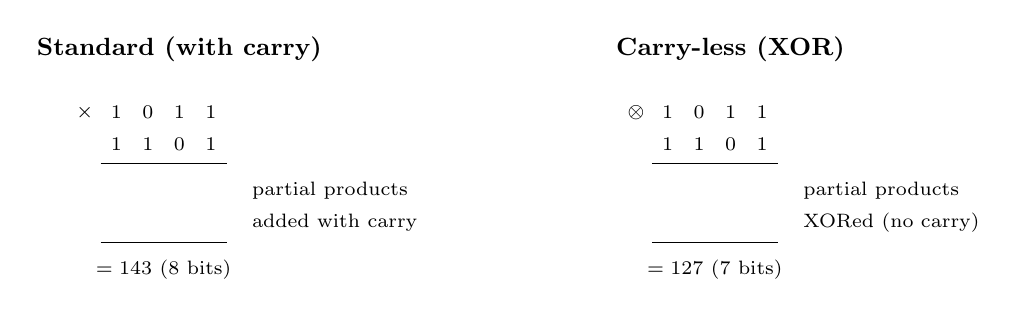
\begin{tikzpicture}[
    >=Latex,
    bit/.style={minimum width=0.4cm, minimum height=0.4cm, font=\scriptsize},
    label/.style={font=\small}
]
% Standard multiplication example: 1011 × 1101
\begin{scope}[shift={(-3.5,0)}]
    \node[label] at (0.8,1.8) {\textbf{Standard (with carry)}};
    \node[bit] at (0,1) {1}; \node[bit] at (0.4,1) {0}; \node[bit] at (0.8,1) {1}; \node[bit] at (1.2,1) {1};
    \node[bit] at (-0.4,1) {$\times$};
    \node[bit] at (0,0.6) {1}; \node[bit] at (0.4,0.6) {1}; \node[bit] at (0.8,0.6) {0}; \node[bit] at (1.2,0.6) {1};
    \draw (-0.2,0.35) -- (1.4,0.35);
    \node[font=\scriptsize, right] at (1.6,0) {partial products};
    \node[font=\scriptsize, right] at (1.6,-0.4) {added with carry};
    \draw (-0.2,-0.65) -- (1.4,-0.65);
    \node[font=\scriptsize] at (0.6,-1) {$= 143$ (8 bits)};
\end{scope}

% Carry-less multiplication
\begin{scope}[shift={(3.5,0)}]
    \node[label] at (0.8,1.8) {\textbf{Carry-less (XOR)}};
    \node[bit] at (0,1) {1}; \node[bit] at (0.4,1) {0}; \node[bit] at (0.8,1) {1}; \node[bit] at (1.2,1) {1};
    \node[bit] at (-0.4,1) {$\otimes$};
    \node[bit] at (0,0.6) {1}; \node[bit] at (0.4,0.6) {1}; \node[bit] at (0.8,0.6) {0}; \node[bit] at (1.2,0.6) {1};
    \draw (-0.2,0.35) -- (1.4,0.35);
    \node[font=\scriptsize, right] at (1.6,0) {partial products};
    \node[font=\scriptsize, right] at (1.6,-0.4) {XORed (no carry)};
    \draw (-0.2,-0.65) -- (1.4,-0.65);
    \node[font=\scriptsize] at (0.6,-1) {$= 127$ (7 bits)};
\end{scope}
\end{tikzpicture}
\end{center}

\noindent
The PCLMULQDQ instruction performs 64$\times$64$\to$128 carry-less multiplication
in a single cycle on modern CPUs.

\paragraph{Pseudocode primitives.}
\label{sec:clmul-primitives}
\begin{align}
\Clmul(a, b) &= a \otimes b \quad\text{(128-bit carry-less product of two 64-bit inputs)}
\end{align}
Both map to a single \texttt{PCLMULQDQ} instruction with $\sim$1~cycle throughput.
The symbol $\otimes$ denotes polynomial multiplication in $\mathrm{GF}(2)[x]$ (XOR replaces addition, AND replaces multiplication of coefficients).

\subsection{CLHash}
\label{sec:clhash}

Source: \href{https://gitlab.com/fwojcik/smhasher3/-/blob/main/hashes/clhash.cpp}{\texttt{hashes/clhash.cpp}}~\cite{clhash}.

\paragraph{SMHasher3 test results.}
CLHash fails 186 of 250 tests, the worst result of any hash in this survey.
Failures span nearly every category: Avalanche, BIC, Sparse, Permutation, Text,
TwoBytes, PerlinNoise, Bitflip, and extensive seed-related tests.
Many seed-test failures are expected: CLHash is a keyed hash designed for a full random
key, and SMHasher3's seed-sensitivity tests probe a regime outside its design model.
The non-seed failures (Avalanche, Sparse, Text) indicate that the CLMUL-based
compression without a strong finalizer leaves detectable bias in the output.

A theoretically-grounded hash by Daniel Lemire using carry-less multiplication (CLMUL instruction,
x86-64 Haswell+). Based on almost-universal hashing over $\mathrm{GF}(2^{127})$ with collision
bound $\epsilon \approx n/2^{64}$. Uses 133 random 64-bit keys derived from seed.

\subsubsection{Mathematical Foundation}

CLHash computes a polynomial hash over $\mathrm{GF}(2^{127})$ with irreducible polynomial $p(x) = x^{127} + x + 1$. (Irreducibility over $\mathrm{GF}(2^{128})$ ensures the field structure.)
The core operation is carry-less multiplication:
\begin{equation}
a \otimes b = a \cdot b \mod p(x)
\end{equation}
where $\cdot$ denotes polynomial multiplication in $\mathrm{GF}(2)[x]$ (XOR instead of addition, AND instead of multiplication for coefficients).

\subsubsection{Key Primitives}

\paragraph{\texorpdfstring{Lazy mod $2^{127} + 2 + 1$:}{Lazy mod 2\string^127 + 2 + 1:}}
Given 254-bit product $(A_{\text{hi}}, A_{\text{lo}})$:
\begin{equation}
A_{\text{lo}} \oplus (A_{\text{hi}} \ll 1) \oplus (A_{\text{hi}} \ll 2)
\end{equation}

\paragraph{128-to-64 reduction:}
Uses the irreducible polynomial $p(x) = x^{64} + x^4 + x^3 + x + 1$ (notation: $(64, 4, 3, 1, 0)$).
The reduction is performed in two steps:

\textbf{Step 1: CLMUL reduction.}
Let $C = x^4 + x^3 + x + 1$ (the low-degree terms of $p(x)$). Since $x^{64} \equiv C \pmod{p(x)}$,
we have $A_{\text{hi}} \cdot x^{64} \equiv A_{\text{hi}} \cdot C$:
\begin{equation}
Q_2 \gets \Clmul(A_{\text{hi}}, C)
\end{equation}
This produces a result up to $64 + 4 = 68$ bits (since $A_{\text{hi}}$ is 64 bits and $C$ is degree 4).

\textbf{Step 2: Table lookup for final bits.}
The CLMUL result $Q_2$ may have bits in positions 64--67. These are reduced using
a precomputed 16-entry table where entry $i$ contains $i \cdot C \bmod 2^{64}$:
\begin{center}
\begin{tabular}{c cccccccc}
\toprule
$i$ & 0 & 1 & 2 & 3 & 4 & 5 & 6 & 7 \\
$i \cdot C$ & 0 & 27 & 54 & 45 & 108 & 119 & 90 & 65 \\
\midrule
$i$ & 8 & 9 & 10 & 11 & 12 & 13 & 14 & 15 \\
$i \cdot C$ & 216 & 195 & 238 & 245 & 180 & 175 & 130 & 153 \\
\bottomrule
\end{tabular}
\end{center}
The high 4 bits of $Q_2$ (bits 64--67) index into this table via \texttt{pshufb}:
\begin{equation}
Q_3 \gets \mathit{table}[(Q_2 \gg 64) \land \texttt{0xF}]
\end{equation}

\textbf{Final combination:}\phantomsection\label{fn:precomp-reduction64}
\begin{equation}
\textsc{precompReduction64}(A) = A_{\text{lo}} \oplus Q_2 \oplus Q_3
\end{equation}
The table lookup replaces what would otherwise require another CLMUL for the
overflow bits, saving one instruction in the critical path.

\subsubsection{CLHash Algorithm}

\begin{algorithmic}[1]
\State Generate 133 random 64-bit key words $s_0, \ldots, s_{132}$ from seed using xorshift128+
\State $s_{\mathrm{poly}} \gets (s_{128} \mid s_{129} \ll 64) \land (\texttt{0x3FFFFFFF\,FFFFFFFF\,FFFFFFFF\,FFFFFFFF})$ \Comment{128-bit; top 2 bits cleared for $\mathrm{GF}(2^{127})$}
\State $s_{\mathrm{final}} \gets (s_{130}, s_{131}) \in \ut{128}$; \quad $s_{\mathrm{len}} \gets s_{132} \in \ut{64}$
\State $v \gets 0$ (128-bit)
\For{each block $(x_i)_{i=0}^{127} \in \ut{64}^{128}$} \Comment{1024 bytes; Horner: $v \gets v \otimes s_{\mathrm{poly}} \oplus h_i$}
    \If{not first block}
        \State $v \gets v \otimes s_{\mathrm{poly}}$
    \EndIf
    \For{$i \in \{0, \ldots, 63\}$} \Comment{64 word pairs}
        \State $v \gets v \oplus \Clmul((x_{2i} \oplus s_{2i}), (x_{2i+1} \oplus s_{2i+1}))$
    \EndFor
\EndFor
\For{remaining word pairs $(x_{2i}, x_{2i+1})$} \Comment{Tail: same CLMUL pattern}
    \State $v \gets v \oplus \Clmul((x_{2i} \oplus s_{2i}), (x_{2i+1} \oplus s_{2i+1}))$
\EndFor
\State $t \gets v \oplus s_{\mathrm{final}}$; \quad $v \gets \Clmul(\textsc{Lo}(t),\, \textsc{Hi}(t))$
\State $v \gets v \oplus \Clmul(s_{\mathrm{len}}, n)$ \Comment{Mix in length}
\State \Return $\hyperref[fn:precomp-reduction64]{\textsc{precompReduction64}}(v)$ \Comment{bitmix variant applies MurmurHash3 $\Fmix$ after}
\end{algorithmic}

\subsection{UMASH}
\label{sec:umash}

Source: \href{https://gitlab.com/fwojcik/smhasher3/-/blob/main/hashes/umash.cpp}{\texttt{hashes/umash.cpp}}~\cite{umash}.

\paragraph{SMHasher3 test results.}
UMASH-128 fails 128 of 250 tests.
Like CLHash, UMASH is a keyed hash expecting a full random key (generated via Salsa20),
and most failures are in seed-related tests (Seed, SeedSparse, SeedAvalanche, SeedBIC,
SeedBitflip, SeedBlockLen, SeedBlockOffset).
Non-seed failures include BIC, some Sparse configurations, Permutation (single-bit keys),
TwoBytes, PerlinNoise, and Bitflip---reflecting the inherent linearity of
CLMUL-based compression.

UMASH by Paul Khuong combines CLMUL-based compression with polynomial hashing
over $\mathrm{GF}(2^{61}-1)$. It produces two independent hash functions for
fingerprinting (128-bit output).

\subsubsection{Mathematical Foundation}

UMASH works modulo the Mersenne prime $p = 2^{61} - 1$. Key operations:

\paragraph{Modular addition (fast):}
\begin{equation}
\textsc{add\_mod\_fast}(x, y) = \begin{cases}
x + y + 8 & \text{if } x + y \text{ overflows} \\
x + y & \text{otherwise}
\end{cases}
\end{equation}

\paragraph{Modular multiplication:}
\begin{equation}
\textsc{mul\_mod\_fast}(m, x) = \textsc{add\_mod\_fast}(\textsc{Lo}(m \times x), 8 \cdot \textsc{Hi}(m \times x))
\end{equation}

\paragraph{Horner double update:}\phantomsection\label{fn:horner-double-update}
\begin{equation}
\begin{aligned}
\textsc{horner\_double\_update}(v, m_0, m_1, x, y) &=
\textsc{mul\_mod\_fast}(m_0, v + x) \\
&\quad + \textsc{mul\_mod\_fast}(m_1, y)
\end{aligned}
\end{equation}

\subsubsection{OH Compression}

The ``OH'' (One-pass Hash) compresses 256-byte blocks using CLMUL:

\phantomsection\label{fn:oh-compress}%
\begin{algorithmic}[1]
\State Interpret the 256-byte input as $(x_i)_{i=0}^{31} \in \ut{64}^{32}$
\State $v \gets 0$ (128-bit)
\For{$i \in \{0, \ldots, 14\}$} \Comment{15 CLMUL pairs}
    \State $v \gets v \oplus \Clmul(x_{2i} \oplus s_{2i}, x_{2i+1} \oplus s_{2i+1})$
\EndFor
\State \textbf{ENH finalization:}
\State $(t_0, t_1) \gets (x_{30} + s_{30},\, x_{31} + s_{31})$ \Comment{Final ENH chunk}
\State $t_2 \gets \textsc{Hi}(t_0 \times t_1) + \mathit{seed}$; $t_3 \gets \textsc{Lo}(t_0 \times t_1)$
\State \Return $(v_{\text{lo}} \oplus t_3,\, v_{\text{hi}} \oplus t_2 \oplus t_3)$
\end{algorithmic}

\subsubsection{UMASH Algorithm}

\noindent We focus on the main (long-key) structure. Short-key special casing and exact tail handling are summarized.

\begin{algorithmic}[1]
\State Generate 34 random 64-bit key words $s_0, \ldots, s_{33}$ from seed via Salsa20
\State Prepare polynomial multipliers $f, f^2$ in $\mathrm{GF}(2^{61}-1)$
\State $v \gets 0$
\For{each block $(x_i)_{i=0}^{31} \in \ut{64}^{32}$} \Comment{Main loop (256 bytes)}
    \State $(t_0, t_1) \gets \hyperref[fn:oh-compress]{\textsc{OH\_compress}}((x_i)_{i=0}^{31})$
    \State $v \gets \hyperref[fn:horner-double-update]{\textsc{horner\_double\_update}}(v, f^2, f, t_0, t_1)$
\EndFor
\State Process remaining bytes with variable-length OH (tail summarized)
\State \Return $(v \oplus \Rot{8}{v}) \oplus \Rot{33}{v}$ \Comment{Finalization}
\end{algorithmic}

\subsubsection{Fingerprinting (128-bit)}

For fingerprinting, UMASH computes two independent hashes using:
\begin{itemize}
\item Different polynomial multipliers $(f_0, f_0^2)$ and $(f_1, f_1^2)$
\item A ``twisted'' version using an LRC (longitudinal redundancy check) XOR~\cite{umash-twist}
\item Both hashes use the same OH keys but different polynomial accumulators
\end{itemize}

\subsection{Polymur}
\label{sec:polymur}

Source: \href{https://gitlab.com/fwojcik/smhasher3/-/blob/main/hashes/polymur.cpp}{\texttt{hashes/polymur.cpp}}~\cite{polymur}.

Polymur by Orson Peters is a polynomial hash over $\mathrm{GF}(2^{61}-1)$. Uses 56-bit
chunks to avoid reduction within chunk processing. The polynomial multiplier $s_0$ is chosen as a generator of the
multiplicative group (via $s_0 = 37^e$ for random odd $e$ coprime to $2^{61}-2$), with
$s_0^7 < 2^{60} - 2^{56}$ ensuring efficient reduction.

\begin{algorithmic}[1]
\State Keys: $(s_0, s_1) \gets$ secret parameters derived from seed \Comment{$s_0$ multiplier, $s_1$ tweak}
\State $v \gets 0$
\If{$n \leq 7$}
		    \State \Return $s_1 + (s_0 + x_0)(s_0^2 + n) \mod p$
\ElsIf{$n \geq 50$}
		    \While{$n \geq 50$} \Comment{Main loop: 7$\times$56-bit chunks per iteration}
		        \State Let $(x_0, \ldots, x_6)$ be the next 7 words (each 56 bits, zero-extended)
		        \State $t_0 \gets (s_0 + x_0)(s_0^6 + x_1)$
		        \State $t_1 \gets (s_0^2 + x_2)(s_0^5 + x_3)$
	        \State $t_2 \gets (s_0^3 + x_4)(s_0^4 + x_5)$
	        \State $t_3 \gets (v + x_6) \cdot s_0^7$
	        \State $v \gets (t_0 + t_1 + t_2 + t_3) \mod p$
	    \EndWhile
		    \State Finalize with $v \cdot s_0^{14}$
\EndIf
\State Handle tail (8--49 bytes) with overlapping reads
\State $s_2 \gets \texttt{0xe9846af9b1a615d}$ \Comment{mx3 finalizer}
\State $v \gets \Xorshift{32}(v) \cdot s_2$
\State $v \gets \Xorshift{32}(v) \cdot s_2$
\State $v \gets \Xorshift{28}(v)$
\State \Return $v + s_1$
\end{algorithmic}

\subsection{poly-mersenne}
\label{sec:poly-mersenne}

Source: \href{https://gitlab.com/fwojcik/smhasher3/-/blob/main/hashes/poly_mersenne.cpp}{\texttt{hashes/poly\_mersenne.cpp}}~\cite{poly-mersenne}.

A simple polynomial hash over the Mersenne prime $p = 2^{61}-1$. Outputs 32 bits.
Keys from SplitMix64: multiplier $s_0 < 2^{60}$ and random values $s_1, \ldots, s_{K+1}$ for
optional $K$-independence.

\paragraph{Core primitive.}\phantomsection\label{fn:mult-combine61}
The multiply-accumulate uses \emph{lazy Mersenne reduction}: since $2^{61} \equiv 1 \pmod{p}$,
a 128-bit product can be reduced by folding the bits above position~61 back into the low part
with a shift and add---no division required.

\begin{algorithmic}[1]
\Function{mult\_combine61}{$v, m, x$} \Comment{$(v \cdot m + x) \bmod (2^{61}-1)$}
    \State $(\mathit{lo}, \mathit{hi}) \gets v \times m$ \Comment{Full 128-bit product}
    \State $\mathit{lo} \gets \mathit{lo} + x$ \Comment{Accumulate input word}
    \State $t \gets (\mathit{hi} \ll 3) \mid (\mathit{lo} \gg 61)$ \Comment{Bits $\geq 2^{61}$: fold back}
    \State $\mathit{lo} \gets \mathit{lo} \land (2^{61}-1)$
    \State \Return $\mathit{lo} + t$ \Comment{Lazy: may exceed $p$ by at most 1}
\EndFunction
\end{algorithmic}

\noindent The final result is fully reduced ($v \gets v - p$ if $v \geq p$) once, after all rounds.

\begin{algorithmic}[1]
\State $v \gets n$ \Comment{Initialize with length}
\For{each word $x \in \ut{32}$}
    \State $v \gets \hyperref[fn:mult-combine61]{\textsc{mult\_combine61}}(v, s_0, x)$
\EndFor
\If{$K > 0$} \Comment{Optional $K$-independence transform}
    \State $t \gets v$; $v \gets s_1$
    \For{$i \in \{2, \ldots, K+1\}$}: $v \gets \hyperref[fn:mult-combine61]{\textsc{mult\_combine61}}(v, t, s_i)$
    \EndFor
\EndIf
\State \Return $v \bmod 2^{32}$ \Comment{After final reduction if $v \geq p$}
\end{algorithmic}

\noindent Variants with higher $K$ provide $K$-wise independence (collision bound $(n/2^{61})^{K+1}$):

\begin{center}
\begin{tabular}{lcc}
\toprule
Variant & $K$ & Collision bound \\
\midrule
poly-mersenne-deg0 & 0 & $n / 2^{61}$ \\
poly-mersenne-deg1 & 1 & $(n / 2^{61})^2$ \\
poly-mersenne-deg2 & 2 & $(n / 2^{61})^3$ \\
poly-mersenne-deg3 & 3 & $(n / 2^{61})^4$ \\
poly-mersenne-deg4 & 4 & $(n / 2^{61})^5$ \\
\bottomrule
\end{tabular}
\end{center}

Higher-degree variants provide $K$-wise independence at the cost of additional
multiplications, improving theoretical collision bounds.

%=============================================================================
\section{AES-Based Hashes}
\label{sec:aes}
%=============================================================================

These hashes leverage the AES-NI instructions (\texttt{aesenc}, \texttt{aesdec})
for fast mixing. AES provides excellent diffusion in a single instruction.

\paragraph{AES round structure.}
Each \texttt{aesenc} instruction applies three transformations to a 128-bit state,
then XORs a round key:

\begin{center}
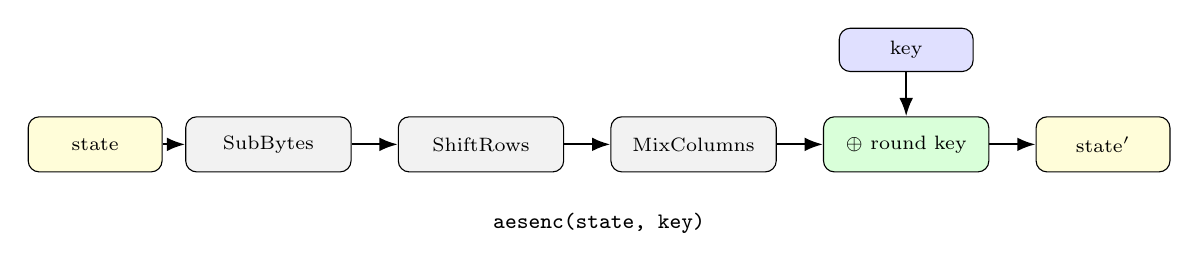
\begin{tikzpicture}[
    >=Latex,
    box/.style={rectangle, draw, rounded corners, minimum width=2.1cm, minimum height=0.7cm, font=\scriptsize, fill=gray!10},
    state/.style={rectangle, draw, rounded corners, minimum width=1.7cm, minimum height=0.7cm, font=\scriptsize, fill=yellow!15},
    key/.style={rectangle, draw, rounded corners, minimum width=1.7cm, minimum height=0.55cm, font=\scriptsize, fill=blue!12},
    arrow/.style={->, thick}
]
\node[state] (in) at (-2.2,0) {state};
\node[box] (sb) at (0,0) {SubBytes};
\node[box] (sr) at (2.7,0) {ShiftRows};
\node[box] (mc) at (5.4,0) {MixColumns};
\node[box, fill=green!15] (xor) at (8.1,0) {$\oplus$ round key};
\node[state] (out) at (10.6,0) {state$'$};

\node[key] (rk) at (8.1,1.2) {key};
\draw[arrow] (rk) -- (xor);

\draw[arrow] (in) -- (sb);
\draw[arrow] (sb) -- (sr);
\draw[arrow] (sr) -- (mc);
\draw[arrow] (mc) -- (xor);
\draw[arrow] (xor) -- (out);

\node[font=\footnotesize] at (4.2,-1.0) {\texttt{aesenc(state, key)}};
\end{tikzpicture}
\end{center}

\paragraph{State transformations.}
The AES state is a 4$\times$4 matrix of bytes. ShiftRows and MixColumns provide
diffusion across the entire state:

\begin{center}
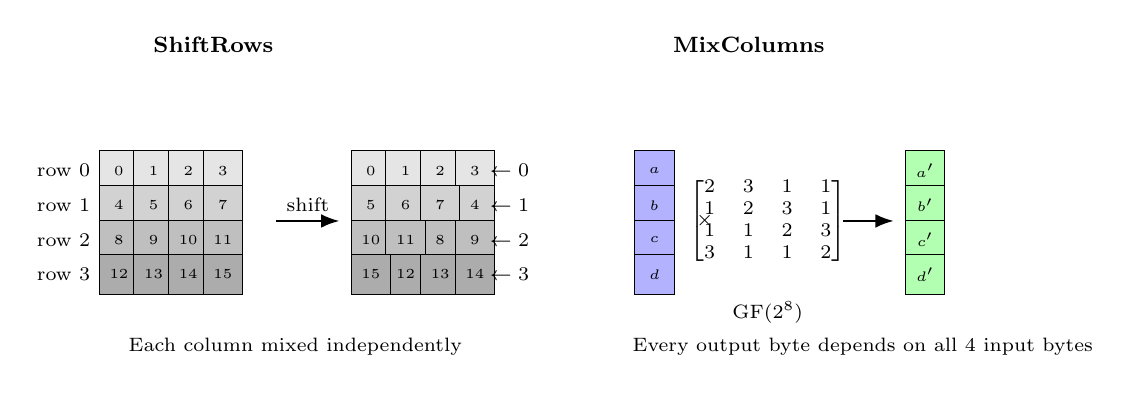
\begin{tikzpicture}[
    >=Latex,
    scale=0.8,
    cell/.style={rectangle, draw, minimum width=0.5cm, minimum height=0.5cm, font=\tiny},
    label/.style={font=\scriptsize}
]
% === ShiftRows ===
\node[label, font=\footnotesize\bfseries] at (1.5, 2) {ShiftRows};

% Input state
\foreach \row in {0,...,3} {
    \foreach \col in {0,...,3} {
        \pgfmathtruncatemacro{\idx}{\row*4+\col}
        \node[cell, fill=gray!\the\numexpr20+\row*15\relax] (in\row\col) at (\col*0.55, -\row*0.55) {\idx};
    }
}
% Row labels
\node[label, anchor=east] at (-0.3, 0) {row 0};
\node[label, anchor=east] at (-0.3, -0.55) {row 1};
\node[label, anchor=east] at (-0.3, -1.1) {row 2};
\node[label, anchor=east] at (-0.3, -1.65) {row 3};

% Arrow
\draw[->, thick] (2.5, -0.8) -- (3.5, -0.8);
\node[label, above] at (3, -0.8) {shift};

% Output state (shifted)
\foreach \row/\shift/\shade in {0/0/20, 1/1/35, 2/2/50, 3/3/65} {
    \foreach \col in {0,...,3} {
        \pgfmathtruncatemacro{\idx}{\row*4+\col}
        \pgfmathtruncatemacro{\newcol}{mod(\col+4-\shift,4)}
        \node[cell, fill=gray!\shade] at (4+\newcol*0.55, -\row*0.55) {\idx};
    }
}

% Shift amounts
\node[label] at (6.2, 0) {$\leftarrow 0$};
\node[label] at (6.2, -0.55) {$\leftarrow 1$};
\node[label] at (6.2, -1.1) {$\leftarrow 2$};
\node[label] at (6.2, -1.65) {$\leftarrow 3$};

% === MixColumns ===
\node[label, font=\footnotesize\bfseries] at (10, 2) {MixColumns};

% Input column
\node[cell, fill=blue!30] (mc0) at (8.5, 0) {$a$};
\node[cell, fill=blue!30] (mc1) at (8.5, -0.55) {$b$};
\node[cell, fill=blue!30] (mc2) at (8.5, -1.1) {$c$};
\node[cell, fill=blue!30] (mc3) at (8.5, -1.65) {$d$};

% Matrix multiply symbol
\node[label] at (9.3, -0.8) {$\times$};

% Matrix
\node[label, align=center] at (10.3, -0.8) {$\begin{bmatrix} 2 & 3 & 1 & 1 \\ 1 & 2 & 3 & 1 \\ 1 & 1 & 2 & 3 \\ 3 & 1 & 1 & 2 \end{bmatrix}$};
\node[label] at (10.3, -2.25) {$\mathrm{GF}(2^8)$};

% Arrow
\draw[->, thick] (11.5, -0.8) -- (12.3, -0.8);

% Output column
\node[cell, fill=green!30] (out0) at (12.8, 0) {$a'$};
\node[cell, fill=green!30] (out1) at (12.8, -0.55) {$b'$};
\node[cell, fill=green!30] (out2) at (12.8, -1.1) {$c'$};
\node[cell, fill=green!30] (out3) at (12.8, -1.65) {$d'$};

% Explanation
\node[label, align=left, anchor=west] at (0, -2.8) {Each column mixed independently};
\node[label, align=left, anchor=west] at (8, -2.8) {Every output byte depends on all 4 input bytes};
\end{tikzpicture}
\end{center}

\noindent
\textbf{SubBytes}: Non-linear S-box substitution (each byte independently).
\textbf{ShiftRows}: Rotates each row by different amounts (0, 1, 2, 3 positions left).
\textbf{MixColumns}: Multiplies each 4-byte column by a fixed matrix in $\mathrm{GF}(2^8)$.
After one round, each output bit depends on multiple input bits---full avalanche
requires $\sim$2 rounds.

\paragraph{Pseudocode primitives.}
\label{sec:aes-primitives}
We use $\Aesenc$ and $\Aesdec$ as 128-bit $\to$ 128-bit operations throughout:
\begin{align}
\Aesenc(v, k) &= \textsc{MixColumns}(\textsc{ShiftRows}(\textsc{SubBytes}(v))) \oplus k \\
\Aesdec(v, k) &= \textsc{InvMixColumns}(\textsc{InvShiftRows}(\textsc{InvSubBytes}(v))) \oplus k
\end{align}
Each maps to a single x86 instruction (AESENC / AESDEC) with $\sim$1~cycle throughput
and $\sim$4~cycle latency on modern CPUs.

\subsection{AquaHash}
\label{sec:aquahash}

Source: \href{https://gitlab.com/fwojcik/smhasher3/-/blob/main/hashes/aquahash.cpp}{\texttt{hashes/aquahash.cpp}}~\cite{aquahash}.

\paragraph{SMHasher3 test results.}
AquaHash fails 55 of 250 tests.
The main weaknesses are in Sparse tests (18 configurations, including long-key
variants up to 2048 bytes), Permutation (single-bit keys), and several Text patterns.
Some seed-related failures (SeedSparse, SeedBlockLen, Seed) also appear.

AquaHash by J. Andrew Rogers uses \texttt{aesenc} for mixing with 4 parallel
128-bit lanes (512-bit state).
We denote the fixed 128-bit constants used by the reference implementation as $s_0,\ldots,s_4$; $s_4$ is used in the final AES round.

\begin{center}
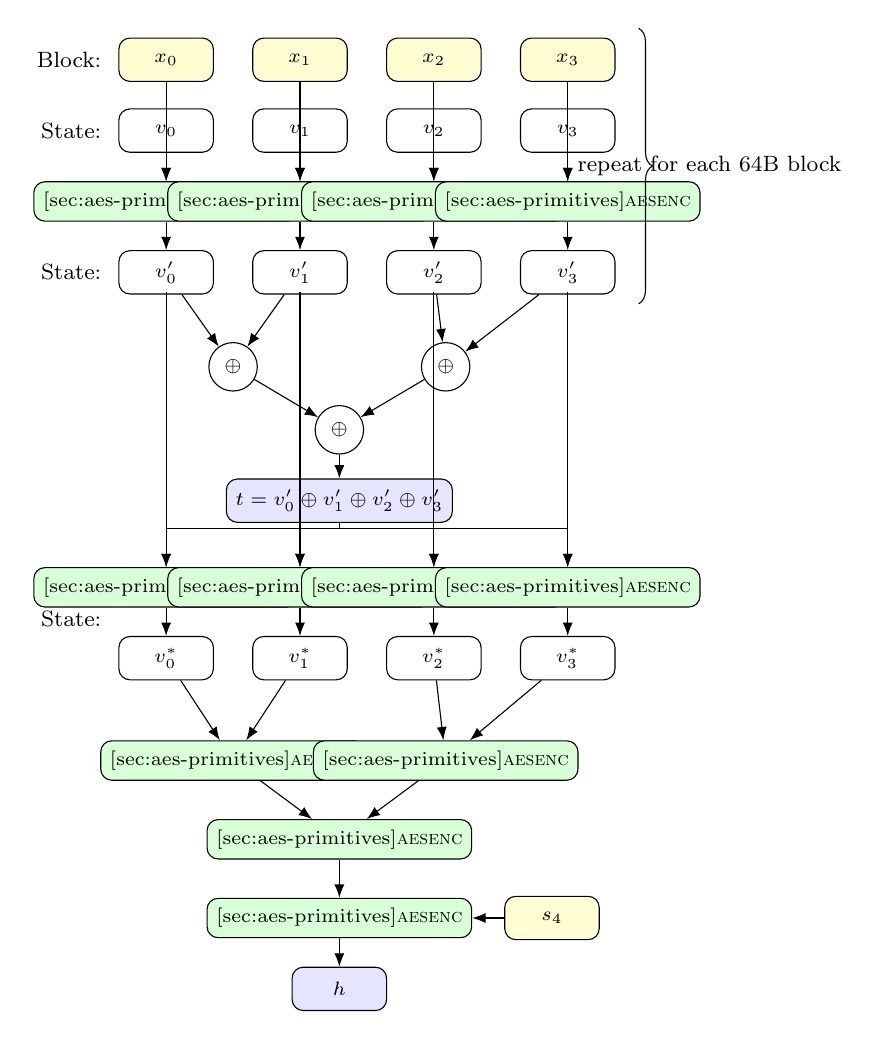
\begin{tikzpicture}[
    >=Latex,
    lane/.style={rectangle, draw, rounded corners, minimum width=1.2cm, minimum height=0.55cm, font=\scriptsize},
    inlane/.style={lane, fill=yellow!18},
    aes/.style={rectangle, draw, rounded corners, minimum width=1.2cm, minimum height=0.5cm, font=\scriptsize, fill=green!15},
    op/.style={circle, draw, minimum size=0.42cm, font=\scriptsize}
]
% Lane x-positions
\def\dx{1.7}

% --- Main loop (per 64-byte block) ---
\node[font=\footnotesize, anchor=east] at (-0.7, 0.0) {Block:};
\node[font=\footnotesize, anchor=east] at (-0.7, -0.9) {State:};
\node[font=\footnotesize, anchor=east] at (-0.7, -2.7) {State:};

\foreach \i in {0,...,3} {
    \pgfmathsetmacro{\x}{\i*\dx}
    \node[inlane] (x\i) at (\x, 0.0) {$x_{\i}$};
    \node[lane] (v\i) at (\x, -0.9) {$v_{\i}$};
    \node[aes] (aes\i) at (\x, -1.8) {\Aesenc};
    \node[lane] (vp\i) at (\x, -2.7) {$v'_{\i}$};
    \draw[->] (x\i) -- (aes\i);
    \draw[->] (v\i) -- (aes\i);
    \draw[->] (aes\i) -- (vp\i);
}
\draw[decorate, decoration={brace, amplitude=5pt}] (6.0, 0.4) -- (6.0, -3.1)
    node[midway, xshift=0.9cm, font=\footnotesize] {repeat for each 64B block};

% --- Lane mix: t = XOR of lanes, then aesenc(v_i, t) ---
\node[op] (xor01) at (0.85, -3.9) {$\oplus$};
\node[op] (xor23) at (3.55, -3.9) {$\oplus$};
\node[op] (xorAll) at (2.2, -4.7) {$\oplus$};
\draw[->] (vp0) -- (xor01);
\draw[->] (vp1) -- (xor01);
\draw[->] (vp2) -- (xor23);
\draw[->] (vp3) -- (xor23);
\draw[->] (xor01) -- (xorAll);
\draw[->] (xor23) -- (xorAll);
\node[lane, fill=blue!10] (t) at (2.2, -5.6) {$t = v_0' \oplus v_1' \oplus v_2' \oplus v_3'$};
\draw[->] (xorAll) -- (t);

\node[font=\footnotesize, anchor=east] at (-0.7, -7.1) {State:};
\foreach \i in {0,...,3} {
    \pgfmathsetmacro{\x}{\i*\dx}
    \node[aes] (aesMix\i) at (\x, -6.7) {\Aesenc};
    \node[lane] (vs\i) at (\x, -7.6) {$v^*_{\i}$};
    \draw[->] (vp\i) -- ++(0,-0.25) -| (aesMix\i);
    \draw[->] (t) -- ++(0,-0.35) -| (aesMix\i);
    \draw[->] (aesMix\i) -- (vs\i);
}

% --- Reduction to one 128-bit output ---
\node[aes] (r01) at (0.85, -8.9) {\Aesenc};
\node[aes] (r23) at (3.55, -8.9) {\Aesenc};
\draw[->] (vs0) -- (r01);
\draw[->] (vs1) -- (r01);
\draw[->] (vs2) -- (r23);
\draw[->] (vs3) -- (r23);
\node[aes] (r0123) at (2.2, -9.9) {\Aesenc};
\draw[->] (r01) -- (r0123);
\draw[->] (r23) -- (r0123);
\node[aes] (final) at (2.2, -10.9) {\Aesenc};
\node[inlane] (sf) at (4.9, -10.9) {$s_4$};
\draw[->] (sf) -- (final);
\draw[->] (r0123) -- (final);
\node[lane, fill=blue!10] (out) at (2.2, -11.8) {$h$};
\draw[->] (final) -- (out);
\end{tikzpicture}
\end{center}

\paragraph{Short keys ($n < 64$):} Uses 2 parallel lanes with \Aesenc, combining via $\Aesenc(v_0, v_1)$ before a 3-round finalization.

\paragraph{Long keys ($n \geq 64$).}

\begin{algorithmic}[1]
\State $(v_0, v_1, v_2, v_3) \gets (\mathit{seed} \oplus s_0, \mathit{seed} \oplus s_1, \mathit{seed} \oplus s_2, \mathit{seed} \oplus s_3)$
\For{each block $(x_0, x_1, x_2, x_3)\in \ut{128}^4$} \Comment{64 bytes}
    \For{$i \in \{0,\ldots,3\}$}
        \State $v_i \gets \Aesenc(v_i, x_i)$
    \EndFor
\EndFor
\State Process remaining 32, 16, 8, 4, 2, 1 bytes
\State $t \gets v_0 \oplus v_1 \oplus v_2 \oplus v_3$
\For{$i \in \{0,\ldots,3\}$}
    \State $v_i \gets \Aesenc(v_i, t)$
\EndFor
\State $v \gets \Aesenc(\Aesenc(v_0, v_1), \Aesenc(v_2, v_3))$
\State \Return $\Aesenc(v, s_4)$
\end{algorithmic}

\subsection{MeowHash}
\label{sec:meowhash}

Source: \href{https://gitlab.com/fwojcik/smhasher3/-/blob/main/hashes/meowhash.cpp}{\texttt{hashes/meowhash.cpp}}, version 0.5/calico~\cite{meowhash}.

MeowHash by Casey Muratori (Molly Rocket) uses 8 parallel 128-bit lanes (1024-bit state)
with \texttt{aesdec} for mixing. Processes 256-byte blocks matching cache line boundaries.
High throughput by saturating AES execution units; for inputs $> 256$KB, explicit prefetch
improves performance.

\begin{center}
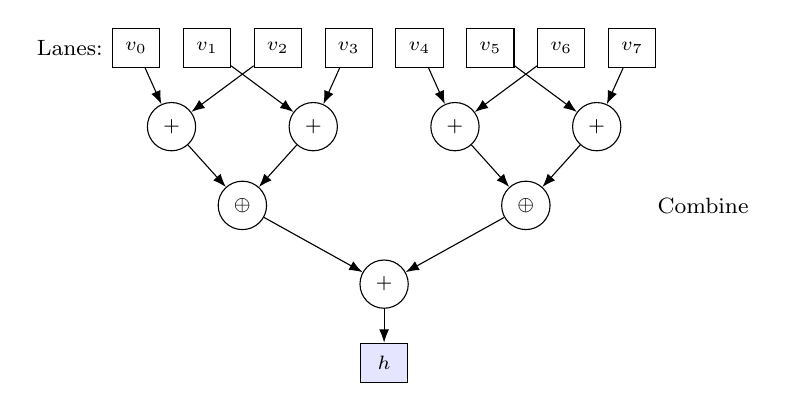
\begin{tikzpicture}[
    >=Latex,
    lane/.style={rectangle, draw, minimum width=0.6cm, minimum height=0.5cm, font=\scriptsize},
    op/.style={circle, draw, minimum size=0.35cm, font=\scriptsize}
]
% 8 lanes
\foreach \i in {0,...,7} {
    \node[lane] (x\i) at (\i*0.9, 0) {$v_\i$};
}
\node[font=\footnotesize, anchor=east] at (-0.3, 0) {Lanes:};

% Final combination tree
% Level 1: additions
\node[op] (a02) at (0.45, -1) {$+$};
\node[op] (a13) at (2.25, -1) {$+$};
\node[op] (a46) at (4.05, -1) {$+$};
\node[op] (a57) at (5.85, -1) {$+$};

\draw[->] (x0) -- (a02);
\draw[->] (x2) -- (a02);
\draw[->] (x1) -- (a13);
\draw[->] (x3) -- (a13);
\draw[->] (x4) -- (a46);
\draw[->] (x6) -- (a46);
\draw[->] (x5) -- (a57);
\draw[->] (x7) -- (a57);

% Level 2: XORs
\node[op] (xor1) at (1.35, -2) {$\oplus$};
\node[op] (xor2) at (4.95, -2) {$\oplus$};

\draw[->] (a02) -- (xor1);
\draw[->] (a13) -- (xor1);
\draw[->] (a46) -- (xor2);
\draw[->] (a57) -- (xor2);

% Level 3: final add
\node[op] (final) at (3.15, -3) {$+$};
\draw[->] (xor1) -- (final);
\draw[->] (xor2) -- (final);

% Output
\node[lane, fill=blue!10] (out) at (3.15, -4) {$h$};
\draw[->] (final) -- (out);

\node[font=\footnotesize, anchor=west] at (6.5, -2) {Combine};
\end{tikzpicture}
\end{center}

\noindent Default seed: 128 bytes from digits of $\pi$.
All additions below are 64-bit lane-wise (\texttt{paddq}).

\phantomsection\label{fn:meow-mix}%
\phantomsection\label{fn:meow-shuffle}%
\begin{algorithmic}[1]
\Function{MEOW\_MIX}{$r_1, r_2, r_3, r_4, r_5, x_a, x_b$} \Comment{32 bytes into 5 lanes}
    \State $r_1 \gets \Aesdec(r_1, r_2)$ \Comment{Source uses 4 overlapping 128-bit reads;}
    \State $r_3 \gets r_3 + x_a$; \quad $r_2 \gets r_2 \oplus x_b$ \Comment{simplified to 2 blocks here}
    \State $r_2 \gets \Aesdec(r_2, r_4)$
    \State $r_5 \gets r_5 + x_a$; \quad $r_4 \gets r_4 \oplus x_b$
\EndFunction
\Function{MEOW\_SHUFFLE}{$r_1, r_2, r_3, r_4, r_5, r_6$} \Comment{Cross-lane mixing (no input)}
    \State $r_1 \gets \Aesdec(r_1, r_4)$
    \State $r_2 \gets r_2 + r_5$; \quad $r_4 \gets r_4 \oplus r_6$
    \State $r_4 \gets \Aesdec(r_4, r_2)$
    \State $r_5 \gets r_5 + r_6$
\EndFunction
\State
\State Initialize 8 lanes $(v_0, \ldots, v_7)$ from 128-byte seed
\For{each block $(x_i)_{i=0}^{15} \in \ut{128}^{16}$} \Comment{Main loop (256 bytes)}
    \For{$i \in \{0,\ldots,7\}$} \Comment{32 bytes per iteration; touches 5 lanes}
        \State $\hyperref[fn:meow-mix]{\textsc{MEOW\_MIX}}(v_i, v_{(i+4)\bmod 8}, v_{(i+6)\bmod 8}, v_{(i+1)\bmod 8}, v_{(i+2)\bmod 8}, x_{2i}, x_{2i+1})$
    \EndFor
\EndFor
\State Load residual $< 32$ bytes with careful alignment handling
\State Mix residual and length into lanes
\State Process remaining 32-byte blocks (0--7)
\State \textbf{MixDown:} Apply 12 \hyperref[fn:meow-shuffle]{\textsc{MEOW\_SHUFFLE}} operations
\State Combine: $v_0 \gets ((v_0 + v_2) \oplus (v_1 + v_3)) + ((v_4 + v_6) \oplus (v_5 + v_7))$
\State \Return $v_0$
\end{algorithmic}

\subsection{aHash}
\label{sec:ahash}

Source: \href{https://gitlab.com/fwojcik/smhasher3/-/blob/main/hashes/rust-ahash.cpp}{\texttt{hashes/rust-ahash.cpp}}~\cite{ahash}.

By Tom Kaitchuck. Default hash in Rust's \texttt{HashMap}. Two variants: AES-based
(2 parallel paths using \texttt{aesdec} + shuffle-add) and fallback (portable MUM-based,
similar to wyhash). Uses variable-amount final rotation for additional mixing.

\paragraph{AES Variant.}
Uses \texttt{aesdec} with a special shuffle permutation (selected by automated search):
\phantomsection\label{fn:ahash-shuffle}\textsc{Shuffle} is a fixed byte permutation of a 128-bit value (as in the implementation).
\begin{algorithmic}[1]
\State $(v_0, v_1) \gets$ state from random seed (derived from $\pi$)
\State $t \gets v_0 \oplus v_1$ \Comment{Save initial combined state}
\For{each block $x \in \ut{128}$}
    \State $v_0 \gets \Aesdec(v_0, x)$
    \State $v_1 \gets \hyperref[fn:ahash-shuffle]{\textsc{Shuffle}}(v_1) + x$
\EndFor
\State $v \gets \Aesenc(v_1, v_0)$
\State \Return $\Aesdec(\Aesdec(v, t), v)$
\end{algorithmic}

\paragraph{Fallback Variant.}
MUM-based, using Knuth's LCG multiplier $s_0 = 6364136223846793005$:

\begin{algorithmic}[1]
\State Initialize $v, s_1, s_2, s_3$ from random state
\State $v \gets \Mum(v \oplus n,\, s_0)$
\State $v \gets (v + n) \cdot s_0$
\For{each block $(x_0, x_1)\in \ut{64}^2$} \Comment{16 bytes}
    \State $t \gets \Mum(x_0 \oplus s_2,\, x_1 \oplus s_3)$
    \State $v \gets (v + s_1) \oplus t$
    \State $v \gets \Rot{23}{v}$
\EndFor
\State \Return $\Rot{v \bmod 64}{\Mum(v,\, s_1)}$
\end{algorithmic}

%=============================================================================
\section{SIMD-Scalable Hashes}
%=============================================================================

\subsection{HalftimeHash}
\label{sec:halftimehash}

Source: \href{https://gitlab.com/fwojcik/smhasher3/-/blob/main/hashes/halftimehash.cpp}{\texttt{hashes/halftimehash.cpp}}~\cite{halftimehash}.

\paragraph{SMHasher3 test results.}
HalftimeHash-128 fails 48 of 250 tests.
The dominant failure category is Sparse (27 configurations including long-key variants),
followed by Permutation (single-bit and low-bit keys) and SeedZeroes.
As a keyed hash requiring ${\sim}50$\,KB of random state, the SeedZeroes failures reflect
SMHasher3's seed model rather than a design flaw.

HalftimeHash by Jim Apple is a SIMD-scalable hash that efficiently uses any vector width
(64-bit scalar to 512-bit AVX-512). Based on erasure coding theory for provable mixing
properties. Uses 32-bit multiplies (\texttt{\_mm\_mul\_epu32}), a tree structure for long
inputs, and requires $\sim$50KB of random state.

The core mixing uses $\textsc{Times}(a, b) = (a \land \texttt{0xFFFFFFFF}) \times (b \land \texttt{0xFFFFFFFF})$
within 64-bit lanes. The Mix function computes
$v + \textsc{Times}(t, t \gg 32)$
where $t = s +_{32} x$ (independent 32-bit lane addition, no carry between halves).

Erasure coding (like RAID) achieves strong mixing: input blocks are encoded with redundancy
(e.g., Encode2: $6 \to 7$ blocks), then reduced using weighted sums.
	For long inputs, a tree structure with fanout 8 combines block groups via depth-first traversal.
	Style variants select block size: Style64 (scalar), Style128 (SSE2/NEON), Style256 (AVX2), Style512 (AVX-512).
	Output is finalized using byte-level tabulation:
	$\mathit{result} = \textsc{TabulateBytes}(n) \oplus \bigoplus_{j} \textsc{TabulateBytes}(h_j)$,
	where $(h_j)$ are the final 64-bit output words for the chosen variant.

\begin{algorithmic}[1]
\phantomsection\label{fn:halftime-mix}%
\Function{Mix}{$v, x, s$} \Comment{Core mixing per block}
    \State $t \gets s +_{32} x$ \Comment{32-bit lane addition}
    \State \Return $v + \textsc{Times}(t, t \gg 32)$ \Comment{$\textsc{Times}$: 32$\times$32 low-half multiply}
\EndFunction
\phantomsection\label{fn:halftime-combine}%
\Function{Combine}{$u_0,\ldots,u_{d'-1}$} \Comment{Fixed linear reducer (variant-specific)}
    \State Compute $(y_0,\ldots,y_{L-1})$ as weighted sums (dot products) of the $u_i$
    \State \Return $(y_0,\ldots,y_{L-1})$
\EndFunction
\phantomsection\label{fn:halftime-baselayer}%
\Function{BaseLayer}{input block group, $s$}
    \State Encode $d$ input blocks into $d'$ blocks via erasure code (XOR-based)
    \State Hash each encoded block into one value $u_i$ using repeated \hyperref[fn:halftime-mix]{\textsc{Mix}} (details elided)
    \State \Return $\hyperref[fn:halftime-combine]{\textsc{Combine}}(u_0,\ldots,u_{d'-1})$
\EndFunction
\phantomsection\label{fn:halftime-upperlayer}%
\Function{UpperLayer}{$(u^{(0)}_0,\ldots,u^{(0)}_{L-1}),\ldots,(u^{(7)}_0,\ldots,u^{(7)}_{L-1}), s$}
    \For{$i \in \{0,\ldots,L-1\}$}
        \State $y_i \gets u^{(0)}_i$
        \For{$j \in \{1,\ldots,7\}$}
            \State $y_i \gets \hyperref[fn:halftime-mix]{\textsc{Mix}}(y_i, u^{(j)}_i, s_{i,j})$
        \EndFor
    \EndFor
    \State \Return $(y_0,\ldots,y_{L-1})$
\EndFunction
\phantomsection\label{fn:halftime-tabulatebytes}%
\Function{TabulateBytes}{$x, T$} \Comment{$T$ is an 8$\times$256 table}
    \State $r \gets 0$
    \For{$i \in \{0,\ldots,7\}$}
        \State $r \gets r \oplus T[i][\mathit{byte}_i(x)]$
    \EndFor
    \State \Return $r$
\EndFunction
\State
\State Let $L \in \{2,3,4,5\}$ be the number of output words (variant-specific)
\State $\mathit{stack}[0 \ldots 8]$ $\gets$ empty \Comment{Tree with fanout 8; each entry is a tuple in $\ut{w}^L$}
\For{each block group in input}
    \State $(y_0,\ldots,y_{L-1}) \gets \hyperref[fn:halftime-baselayer]{\textsc{BaseLayer}}(\text{block group}, s)$
    \State Push $(y_0,\ldots,y_{L-1})$ onto $\mathit{stack}[0]$
    \State $\ell \gets 0$
    \While{$|\mathit{stack}[\ell]| = 8$} \Comment{Collapse full levels}
        \State $(y_0,\ldots,y_{L-1}) \gets \hyperref[fn:halftime-upperlayer]{\textsc{UpperLayer}}(\mathit{stack}[\ell], s)$
        \State Clear $\mathit{stack}[\ell]$; push $(y_0,\ldots,y_{L-1})$ onto $\mathit{stack}[\ell+1]$
        \State $\ell \gets \ell + 1$
    \EndWhile
\EndFor
\State Initialize accumulators $a_0,\ldots,a_{L-1} \gets 0$
\State Let $T^{(0)},\ldots,T^{(L)}$ be 8$\times$256 tables derived from entropy ($T^{(0)}$ for length, $T^{(i+1)}$ for $h_i$)
\State Mix remaining stack tuples and remaining input blocks into $(a_0,\ldots,a_{L-1})$ using \hyperref[fn:halftime-mix]{\textsc{Mix}} (tail summarized)
\State Reduce each accumulator block by summing its 64-bit lanes: $h_i \gets \sum \text{lanes}(a_i)$
\State $r \gets \hyperref[fn:halftime-tabulatebytes]{\textsc{TabulateBytes}}(n, T^{(0)})$
\For{$i \in \{0,\ldots,L-1\}$}
    \State $r \gets r \oplus \hyperref[fn:halftime-tabulatebytes]{\textsc{TabulateBytes}}(h_i, T^{(i+1)})$
\EndFor
\State \Return $r$
\end{algorithmic}

\subsection{khashv}
\label{sec:khashv}

Source: \href{https://gitlab.com/fwojcik/smhasher3/-/blob/main/hashes/khashv.cpp}{\texttt{hashes/khashv.cpp}}~\cite{khashv}.

By Keith-Cancel. A vectorizable hash using S-box byte substitution and SIMD-friendly
shuffles that map to \texttt{pshufb} (SSSE3+). Uses no multiplication---only add, XOR,
rotate, and table lookup. Endian-independent with compact 128-bit state (four 32-bit words,
initialized from SHA-256 hashes of bytes 1--4).

Non-linear mixing uses a nibble-decomposed S-box (similar to AES SubBytes), and
$\textsc{shuffle}$ applies fixed byte permutation $(7,14,9,0,12,15,13,8,5,11,6,3,4,2,10,1)$.

\paragraph{Primitives.}
Two 16-byte lookup tables $S_1, S_2$ define the S-box:
\phantomsection\label{fn:khashv-sbox}%
\phantomsection\label{fn:khashv-rotr5}%
\phantomsection\label{fn:khashv-shuffle}%
\phantomsection\label{fn:khashv-mixwords}%
\begin{algorithmic}[1]
\Function{sbox}{$x$} \Comment{128-bit $\to$ 128-bit, applied per byte}
    \For{each byte $b$ in $x$}
        \State $b \gets S_1[b \land \texttt{0xF}] \oplus S_2[b \gg 4]$ \Comment{Low/high nibble lookup + XOR}
    \EndFor
    \State \Return $x$
\EndFunction
\Function{rotr5}{$v$} \Comment{Rotate 16-byte state right by 5 bytes}
    \State \Return bytes of $v$ permuted: $b_i \gets b_{(i+5) \bmod 16}$
\EndFunction
\Function{shuffle}{$v$} \Comment{Fixed byte permutation (\texttt{pshufb}-style)}
    \State \Return bytes of $v$ permuted: $b_i \gets b_{\pi(i)}$ where $\pi=(7,14,9,0,12,15,13,8,5,11,6,3,4,2,10,1)$
\EndFunction
\Function{mix\_words}{$v$} \Comment{Finalization: operates on 32-bit words}
    \State $v \gets v \oplus (v \gg_{32} 3)$ \Comment{Shift each 32-bit word right by 3, XOR back}
    \For{$r \in (5,\, 7,\, 11,\, 17)$}
        \State $t \gets \hyperref[fn:khashv-rotr5]{\textsc{rotr5}}(v) + v$
        \State $v \gets v \oplus \Rot{r}{t}$ \Comment{Rotate each 32-bit word right by $r$}
    \EndFor
    \State \Return $v$
\EndFunction
\end{algorithmic}

\paragraph{khashv Algorithm.}
\begin{algorithmic}[1]
\State $v \gets \mathit{seed}$ \Comment{128-bit state: four 32-bit words $(v_0, v_1, v_2, v_3)$}
\State $v_0 \gets v_0 \oplus (n \bmod 2^{32})$; \quad $v_1 \gets v_1 \oplus (n \gg 32)$
\For{each block $x \in \ut{128}$}
    \State $t \gets \hyperref[fn:khashv-sbox]{\textsc{sbox}}(x)$
    \State $v \gets v \oplus (t \cdot 8193)$ \Comment{$8193 = 2^{13}+1$}
    \State $v \gets \hyperref[fn:khashv-rotr5]{\textsc{rotr5}}(v) + t$
    \State $v \gets v + \hyperref[fn:khashv-shuffle]{\textsc{shuffle}}(v)$
\EndFor
\State $v \gets \hyperref[fn:khashv-mixwords]{\textsc{mix\_words}}(v)$
\State \Return $v_3$ (32-bit) or $(v_0, v_1)$ (64-bit)
\end{algorithmic}


\appendix
\section{Folded Multiply (\texorpdfstring{$\mathrm{lo}\oplus\mathrm{hi}$}{lo xor hi})}
\label{sec:mum-analysis}

Let $m=2^n$. For each $x\in\{0,1,\dots,m-1\}$, define
\[
\operatorname{op}(x,y) \;=\; \Big\lfloor \frac{xy}{m}\Big\rfloor \;\oplus\; (xy\bmod m),
\]
and fiber sizes
\[
N_x(a) \;=\; \#\{y\in[0,m-1]:\operatorname{op}(x,y)=a\}.
\]
The collision count is
\[
C(x) \;=\; \sum_{a=0}^{m-1} N_x(a)^2,
\qquad
\mathbb{E}[C] \;=\; \frac{1}{m}\sum_{x=0}^{m-1} C(x).
\]

To bound $\mathbb{E}[C]$ we separate the two spike outputs $a=0$ and $a=m-1$ (the only ones amenable to exact analysis) and treat the rest as a residual term:
\[
C(x) = N_x(0)^2 + N_x(m-1)^2 + C^*(x),
\qquad
C^*(x) = \sum_{a\notin\{0,m-1\}} N_x(a)^2.
\]

Below are sharp, self-contained bounds on the \textbf{spike contribution}, plus a rigorous explanation of why ``repeating multipliers'' (like $0101\ldots$) cannot accumulate enough mass to change $\mathbb{E}[C]$ at the $m\log\log n$ scale.

%----------------------------------------------------------------------
\subsection{Exact formulas for the two spike fibers}
\label{sec:spike-fibers}

\begin{lemma}[Exact spike counts]\label{lem:spike-counts}
For $1\le x\le m-1$,
\[
N_x(0) = \gcd(x,\, m+1), \qquad N_x(m-1) = \gcd(x,\, m-1).
\]
\end{lemma}

\begin{proof}
$\operatorname{op}(x,y)=0$ means ``high $=$ low,'' i.e.\ $q=r$ in $xy=mq+r$. Then
\[
xy = mq + q = (m+1)q,
\]
so $(m+1)\mid xy$. Let $d=\gcd(x,m+1)$. Then $(m+1)\mid xy$ is equivalent to $\frac{m+1}{d}\mid y$, because $\gcd(x/d,(m+1)/d)=1$. Since $x<m$, we have $d<m+1$, hence $(m+1)/d\ge 2$, and the multiples of $(m+1)/d$ in $[0,m-1]$ are exactly
\[
0,\; \frac{m+1}{d},\; 2\frac{m+1}{d},\; \dots,\; (d-1)\frac{m+1}{d},
\]
whose last term is $(m+1)-(m+1)/d \le m-1$. So there are exactly $d$ solutions $y$, i.e.\ $N_x(0)=d$.

$\operatorname{op}(x,y)=m-1$ means $q\oplus r = m-1$, which forces $r=(m-1)-q$. Then
\[
xy = mq + r = mq + (m-1-q) = (m-1)(q+1),
\]
so $(m-1)\mid xy$. Let $d=\gcd(x,m-1)$. As above, $(m-1)\mid xy$ is equivalent to $\frac{m-1}{d}\mid y$, and the multiples in $[0,m-1]$ are
\[
0,\; \frac{m-1}{d},\; 2\frac{m-1}{d},\; \dots,\; (d-1)\frac{m-1}{d} = m-1-\frac{m-1}{d} < m,
\]
giving exactly $d$ solutions. So $N_x(m-1)=d$.
\end{proof}

For $x=0$, $\operatorname{op}(0,y)=0$ for all $y$, so $N_0(0)=m$ and $N_0(m-1)=0$. This single $x$ contributes only $O(m)$ to $\mathbb{E}[C]$, so it never affects asymptotics.

%----------------------------------------------------------------------
\subsection{Turning the spike identities into \texorpdfstring{$\Theta(m\log\log n)$}{Theta(m log log n)}}
\label{sec:spike-theta}

We need $\mathbb{E}[N_x(0)^2]$ and $\mathbb{E}[N_x(m-1)^2]$. These are essentially averages of $\gcd(\cdot,N)^2$.

\begin{lemma}[Sum of squared gcds]\label{lem:gcd-sum}
For any $N\ge 1$,
\[
\sum_{k=1}^{N}\gcd(k,N)^2 \;=\; N^2\sum_{d\mid N}\frac{\varphi(d)}{d^2},
\]
where $\varphi$ is Euler's totient.
\end{lemma}

\begin{proof}
Group $k$ by $g=\gcd(k,N)$. Writing $k=gk'$ with $\gcd(k',N/g)=1$, there are $\varphi(N/g)$ such $k$. Hence
\[
\sum_{k=1}^{N}\gcd(k,N)^2
= \sum_{g\mid N} g^2\,\varphi(N/g)
= \sum_{d\mid N}\Big(\frac{N}{d}\Big)^{\!2}\varphi(d)
= N^2\sum_{d\mid N}\frac{\varphi(d)}{d^2}. \qedhere
\]
\end{proof}

Define
\[
F(N) := \sum_{d\mid N}\frac{\varphi(d)}{d^2}.
\]

\begin{lemma}[$F(N)$ versus $\sigma(N)/N$]\label{lem:F-vs-sigma}
Let $\sigma(N)=\sum_{d\mid N} d$. Then for all $N$,
\[
\frac{6}{\pi^2}\cdot\frac{\sigma(N)}{N} \;\le\; F(N) \;\le\; \frac{\sigma(N)}{N}.
\]
\end{lemma}

\begin{proof}
Write $N=\prod p^{e_p}$. Both $F$ and $\sigma(\cdot)/\cdot$ factor over prime powers:
\[
\frac{\sigma(N)}{N} = \prod_{p^e\| N}\Big(1+\frac{1}{p}+\cdots+\frac{1}{p^e}\Big),
\]
and one can compute
\[
F(N) = \prod_{p^e\| N}\Big(1+\frac{1}{p}-\frac{1}{p^{e+1}}\Big).
\]
For each prime power,
\[
1+\frac{1}{p}-\frac{1}{p^{e+1}}
\;\le\; 1+\frac{1}{p}+\cdots+\frac{1}{p^e},
\]
and also
\begin{align*}
1+\frac{1}{p}-\frac{1}{p^{e+1}}
&= \Big(1+\frac{1}{p}+\cdots+\frac{1}{p^e}\Big) - \Big(\frac{1}{p^2}+\cdots+\frac{1}{p^{e+1}}\Big) \\
&\ge \Big(1-\frac{1}{p^2}\Big)\Big(1+\frac{1}{p}+\cdots+\frac{1}{p^e}\Big).
\end{align*}
Multiplying over primes gives
\[
F(N) \;\ge\; \Big(\prod_{p\mid N}\big(1-\tfrac{1}{p^2}\big)\Big)\frac{\sigma(N)}{N}
\;\ge\; \Big(\prod_{p}\big(1-\tfrac{1}{p^2}\big)\Big)\frac{\sigma(N)}{N}
\;=\; \frac{6}{\pi^2}\,\frac{\sigma(N)}{N}. \qedhere
\]
\end{proof}

\paragraph{Consequence for spike second moments.}
\begin{itemize}
\item For $a=m-1$: here $N=m-1$ and $x$ runs through $1,2,\dots,m-1$ exactly, so
  \[
  \frac{1}{m}\sum_{x=1}^{m-1} N_x(m-1)^2
  = \frac{1}{m}\sum_{x=1}^{m-1}\gcd(x,m-1)^2
  = \frac{(m-1)^2}{m}\,F(m-1)
  = \Theta\!\big(\sigma(m-1)\big).
  \]

\item For $a=0$: $N=m+1$ but $x$ only runs up to $m-1=N-2$. Dropping the final two terms only changes the sum by $O(N^2)$, which becomes $O(m)$ after dividing by $m$. So
  \[
  \mathbb{E}[N_x(0)^2] = \Theta\!\big(\sigma(m+1)\big).
  \]
\end{itemize}

Thus the \textbf{spike part of $\mathbb{E}[C]$} is
\[
\mathbb{E}\big[N_x(0)^2 + N_x(m-1)^2\big] = \Theta\!\big(\sigma(2^n+1)+\sigma(2^n-1)\big).
\]

\paragraph{Upper bound $O(m\log\log n)$ for the spike part.}
A theorem of Erd\H{o}s~\cite{erdos1948} gives
\[
\sigma(2^n-1) \;\le\; c\,(2^n-1)\log\log n
\quad\text{for large }n,
\]
for an absolute constant $c$.

To also bound $\sigma(2^n+1)$, observe that
\[
2^{2n}-1 = (2^n-1)(2^n+1), \qquad \gcd(2^n-1,\,2^n+1)=1,
\]
so $\sigma(2^{2n}-1)=\sigma(2^n-1)\,\sigma(2^n+1)$. Applying the same bound at exponent $2n$ gives
\[
\sigma(2^{2n}-1) \le c'(2^{2n}-1)\log\log(2n),
\]
and since $\sigma(2^n-1)\ge 2^n-1$, we get
\[
\sigma(2^n+1) \le \frac{\sigma(2^{2n}-1)}{\sigma(2^n-1)} = O(2^n\log\log n).
\]

Therefore, unconditionally,
\[
\mathbb{E}\big[N_x(0)^2 + N_x(m-1)^2\big] = O(m\log\log n).
\]

\paragraph{Lower bound $\Omega(m\log\log n)$ for infinitely many $n$.}
Take $n=t!$ and $m=2^n$. For every odd prime $p\le t$, we have $p-1\mid t!$, so by Fermat's little theorem $2^{t!}\equiv 1\pmod{p}$, hence $p\mid(2^{t!}-1)$.

Thus $2^{t!}-1$ is divisible by $\prod_{p\le t}p$, so
\[
\frac{\sigma(2^{t!}-1)}{2^{t!}-1} \;\ge\; \prod_{p\le t}\Big(1+\frac{1}{p}\Big).
\]
Now
\[
\prod_{p\le t}\Big(1+\frac{1}{p}\Big)
= \prod_{p\le t}\Big(1-\frac{1}{p^2}\Big)\cdot\prod_{p\le t}\Big(1-\frac{1}{p}\Big)^{-1}.
\]
Mertens' theorem says $\prod_{p\le t}(1-\frac{1}{p})\sim e^{-\gamma}/\log t$, i.e.\ the inverse grows like $e^\gamma\log t$. Also $\prod_{p\le t}(1-\frac{1}{p^2})$ stays bounded below by a positive constant (it converges to $6/\pi^2$). Hence
\[
\prod_{p\le t}\Big(1+\frac{1}{p}\Big) \;\ge\; c\,\log t
\quad\text{for large }t,
\]
so
\[
\sigma(2^{t!}-1) \;\ge\; c\,(2^{t!}-1)\log t.
\]
Since $n=t!$, we have $\log\log n = \log\log(t!) = \Theta(\log t)$. Therefore
\[
\sigma(2^n-1) \;\ge\; c'\,2^n\log\log n
\quad\text{for infinitely many }n,
\]
and since $\mathbb{E}[C]\ge \mathbb{E}[N_x(m-1)^2]=\Theta(\sigma(2^n-1))$, we get
\[
\mathbb{E}[C] = \Omega(m\log\log n)
\quad\text{infinitely often.}
\]

\paragraph{Summary so far (rigorous).}
\[
\mathbb{E}[C] \;=\; \mathbb{E}[C^*] \;+\; O(m\log\log n),
\]
and also $\mathbb{E}[C]\ge \Omega(m\log\log n)$ along the subsequence $n=t!$.
So the entire problem of a tight upper bound is now concentrated in $\mathbb{E}[C^*]$.

%----------------------------------------------------------------------
\subsection{Non-spike outputs: do repeating multipliers matter?}
\label{sec:non-spike}

Outside $\{0,m-1\}$, some $x$'s have noticeably larger fibers $N_x(a)$ (e.g.\ $x=0101\ldots$, which is $x=(m-1)/3$ when $n$ is even). The key point for the expectation is: \textbf{those multipliers form a tiny set}, so they cannot accumulate enough mass to change $\mathbb{E}[C]$ at the $m\log\log n$ scale.

\paragraph{A.\ Any fixed-period family contributes only $O(m)$.}
Fix a period $p$. There are at most $2^p$ $n$-bit strings with period $p$ (choose the length-$p$ template; the rest repeats). For each $x$,
\[
C(x) = \sum_a N_x(a)^2 \;\le\; \Big(\sum_a N_x(a)\Big)^{\!2} = m^2.
\]
So the total contribution of all period-$p$ multipliers to the expectation is
\[
\frac{1}{m}\sum_{\substack{x\text{ has}\\\text{period }p}} C(x) \;\le\; \frac{1}{m}\cdot 2^p \cdot m^2 \;=\; 2^p\,m.
\]
For constant $p$ (like $p=2$ for $0101\ldots$), this is $O(m)$, which is negligible compared to the spike term $m\log\log n$ once $n$ is large.

\paragraph{B.\ The whole divisor family $x\mid(m-1)$ stays at $O(m\log\log n)$.}
This is a more relevant ``big structured class,'' because periodic patterns like $0101\ldots$ are typically divisors of $m-1$ (or closely related).

For any $x$, a trivial but useful bound is
\[
C(x) \le mx,
\]
since for $1\le x\le m-1$ we have $q=\lfloor xy/m\rfloor \in \{0,1,\ldots,x-1\}$, and for a fixed output
$a=q\oplus r$ each choice of $q$ forces $r=a\oplus q$ and hence at most one $y$ solving $xy=mq+r$.
Thus $N_x(a)\le x$, so $C(x)=\sum_a N_x(a)^2 \le (\max_a N_x(a))\sum_a N_x(a)\le x\cdot m$.
so for the divisor family $x\mid(m-1)$,
\[
\frac{1}{m}\sum_{x\mid(m-1)} C(x) \;\le\; \frac{1}{m}\sum_{x\mid(m-1)} mx \;=\; \sigma(m-1) \;=\; O(m\log\log n),
\]
using Erd\H{o}s' bound on $\sigma(2^n-1)$~\cite{erdos1948}.

So \textbf{even if every single divisor of $m-1$} had maximally bad non-spike behavior (it does not), its \emph{total} effect on $\mathbb{E}[C]$ cannot exceed the same $O(m\log\log n)$ scale that the spike already forces.

%----------------------------------------------------------------------
\subsection{What remains for bounding \texorpdfstring{$\mathbb{E}[C]$}{E[C]}}
\label{sec:mum-remaining}

The sharp part of the expectation is now cleanly isolated:
\begin{itemize}
\item The \textbf{only provably growing term} is the spike contribution, and it is
  \[
  \Theta\!\big(\sigma(2^n-1)+\sigma(2^n+1)\big) = O(m\log\log n),
  \]
  with a matching $\Omega(m\log\log n)$ lower bound infinitely often.

\item Repeating multipliers and similar structured classes are provably too sparse to change the leading scale of $\mathbb{E}[C]$.
\end{itemize}

To obtain a full $\mathbb{E}[C]=O(m\log\log n)$ upper bound, the missing ingredient is:
\begin{quote}
Show $\mathbb{E}[C^*]=O(m)$ (or at least $O(m\log\log n)$).
\end{quote}
Empirically $\mathbb{E}[C^*]/m$ appears bounded (it hovers around a small constant for all small $n$), but proving it seems to require a genuine ``mixing'' statement: roughly, that for typical $x$, the non-spike outputs behave like a near-random mapping, so $\sum_{a\ne 0,m-1}N_x(a)^2$ stays $\Theta(m)$.

% Empirical / image-size perspective on the same primitive.
% Empirical appendix for folded multiply.

\subsection{Empirics for folded multiply}
\label{sec:appendix-folded-multiply}

The operation $\operatorname{op}(x,y)=\lfloor xy/m\rfloor \oplus (xy\bmod m)$ can also be viewed,
for fixed $x$, as a map $f_x:\{0,\ldots,m-1\}\to\{0,\ldots,m-1\}$.
We write $m(x)=|\mathrm{Im}(f_x)|$ for its image size.

\paragraph{Image size versus collisions.}
If a function $f$ on an $m$-element domain has image size $M$, then (writing
$C^\mathrm{pairs}=\#\{(a,b):0\le a<b<m,\ f(a)=f(b)\}$) one has
\[
  C^\mathrm{pairs} \ge \frac{1}{2}\left(\frac{m^2}{M}-m\right).
\]
In terms of the ordered-pair statistic used above,
$C(x)=\sum_a N_x(a)^2 = m + 2C^\mathrm{pairs}$.

\paragraph{Variants compared.}
We compare four closely related fold constructions (all returning a $\ut{n}$ value):
\[
  \texttt{nmul\_xor}: \ \mathrm{lo}(xa)\oplus \mathrm{hi}(xa),
  \quad
  \texttt{nmul\_add}: \ (\mathrm{lo}(xa)+\mathrm{hi}(xa))\bmod 2^n,
\]
where $xa$ is ordinary integer multiplication, and
\[
  \texttt{cmul\_xor}: \ \mathrm{lo}(x\otimes a)\oplus \mathrm{hi}(x\otimes a),
  \quad
  \texttt{cmul\_add}: \ (\mathrm{lo}(x\otimes a)+\mathrm{hi}(x\otimes a))\bmod 2^n,
\]
where $x\otimes a$ is carryless (polynomial) multiplication over $\mathbb{F}_2$.

\paragraph{Field baselines.}
In a true field, multiplication by $x\ne 0$ is a permutation, hence has no collisions.
Therefore, for any field of size $N$,
\[
  \mathbb{E}_{x}[C_x] = \frac{1}{N}\binom{N}{2} = \frac{N-1}{2},
  \qquad
  \mathbb{E}_{x}[C_x]/N \approx \frac{1}{2}.
\]
In the plots below we include two baselines: \texttt{gf2n\_field} (a field of size $2^n$, for any
irreducible polynomial of degree $n$) and \texttt{prime\_field} (multiplication modulo the largest
prime $p \le 2^n$).

\paragraph{Carryless \texttt{cmul\_xor} admits an exact collision formula.}
For carryless multiplication, the map $a \mapsto \mathrm{lo}(x\otimes a)\oplus \mathrm{hi}(x\otimes a)$
is multiplication by $x$ in the ring $\mathbb{F}_2[t]/(t^n+1)$. Writing $g=\gcd(x,\,t^n+1)$ and
$d=\deg(g)$, one has $|\ker f_x|=2^d$, $m(x)=2^{n-d}$, and
\[
  C_x = 2^{n-1}(2^d-1).
\]
This explains the strong $n$-dependence seen for \texttt{cmul\_xor}.

\paragraph{Empirical results.}
Figure~\ref{fig:folded-multiply-collisions} shows $\mathbb{E}[C_x]$ and its normalized version
$\mathbb{E}[C_x]/2^n$ for all variants. For \texttt{nmul\_xor} we observe an approximately constant
factor $\mathbb{E}[C_x]/2^n \approx 1.5$--$2.2$ for $n \le 15$ (exact enumeration); for $n>15$ we
estimate using Monte Carlo sampling over multipliers $x$.

\begin{figure}[t]
  \centering
  \includegraphics[width=\linewidth]{scripts/folded_multiply/out/expected_collisions_variants.png}
  \caption{Expected collision pairs $\mathbb{E}[C_x]$ (top) and normalized constant
  $\mathbb{E}[C_x]/2^n$ (bottom) for folded multiply variants.}
  \label{fig:folded-multiply-collisions}
\end{figure}

\paragraph{Achievable \texorpdfstring{$(\delta,\varepsilon)$}{(delta,epsilon)} frontier.}
Define the image-size threshold $M(\delta)=2^{(1-\delta)n}$ and the ``bad multiplier'' event
$m(x)\le M(\delta)$. Let $p_n(\delta)=\Pr_x[m(x)\le M(\delta)]$. The plot in
Figure~\ref{fig:folded-multiply-frontier} shows $p_n(\delta)$ using the more stable $x$-axis
$\Delta=\delta n$ (bits below $n$), which aligns curves across $n$.

\begin{figure}[t]
  \centering
  \includegraphics[width=\linewidth]{scripts/folded_multiply/out/delta_n_fraction_frontier_log.png}
  \caption{Fraction of multipliers with small image: $p_n(\delta)=\Pr_x[m(x)\le 2^{n-\Delta}]$,
  plotted against $\Delta=\delta n$ on a log-$y$ scale (exhaustive for $n\le 15$, sampled after).}
  \label{fig:folded-multiply-frontier}
\end{figure}



\bibliographystyle{alpha}
\bibliography{refs}

\end{document}
